\documentclass[oneside,9pt]{memoir}

% Colors
\usepackage[dvipsnames]{xcolor}
\usepackage[scaled=0.8]{beramono}

% hyperref
\usepackage[%
    colorlinks=true,
    linktocpage=true,
    breaklinks=true,
    linkcolor=NavyBlue,
    urlcolor=NavyBlue,
    citecolor=NavyBlue
]{hyperref}
\def\chapterautorefname{§}
\def\sectionautorefname{§}
\def\subsectionautorefname{§}
\def\subsubsectionautorefname{§}

\setcounter{secnumdepth}{3}


% Fonts
\usepackage{fontspec}
\setmainfont[Numbers = {OldStyle, Proportional}]{TeX Gyre Pagella}

\usepackage{amsmath}
\DeclareMathOperator*{\argmax}{arg\,max}
%\usepackage{amssymb}
\usepackage{unicode-math}
\setmathfont{TeX Gyre Pagella Math}

\usepackage{algorithm}
\usepackage[italicComments=false]{algpseudocodex}

\newcommand{\algorithmautorefname}{Algorithm}

% Typography
\usepackage[tracking]{microtype}

% Images
\usepackage{graphicx}

% ======================================================================
% Memoir package - layout and styling
% ======================================================================

% The calc package is required for calculating readable text widths
\usepackage{calc}

% Set outer and spine margins A wide right margin is chosen both for legibility
% of the typeblock and for tight integration of marginfigures and margin
% footnotes.

% Calculate widths in pts
\setlxvchars[\normalfont\normalsize] % about 66 characters per column
\setxlvchars[\normalfont\footnotesize] % about 45 characters per column

% Set left and right margins
\setlrmarginsandblock{1.15in}{3.5in}{*}
% Set upper and lower margins
\setulmarginsandblock{1.1in}{1.1in}{*}

% Set properties of margin notes, sidecaptioned floats, and footnotes in the
% margin.
\setmarginnotes{0.2in}{2.15in}{2\onelineskip}
\setsidecaps{0.2in}{2.15in}
\sidecapmargin{outer}
\renewcommand*{\sidecapstyle}{\normalfont\footnotesize}
\setsidecappos{c}


% Set footnotes in the margin rather than at the foot of the page
\footnotesinmargin
\setsidefeet{\marginparsep}{1.9in}{0.2in}{0pt}{\flushleftright\footnotesize}{*}

% Integrate the counters of the sidefootnotes and footnotes in margin.
\letcountercounter{sidefootnote}{footnote}
\setlength{\footmarkwidth}{0em}
\setlength{\footmarksep}{-\footmarkwidth}
\setlength{\footparindent}{1em}
\sideparmargin{outer}

\renewcommand*{\sideparfont}{\color{Maroon}\emphshape}
\renewcommand*{\sideparvshift}{2\baselineskip}
\marginparmargin{outer}

% Style the entries in the Table of Contents
\renewcommand*{\cftchapterfont}{\scshape\MakeTextLowercase}
\renewcommand*{\cftpartfont}{\color{Maroon}\scshape\MakeTextLowercase}
\captionstyle[\centering]{\footnotesize}
\captionnamefont{\footnotesize\color{Maroon}}

%% Bringhurst chapter and head styles with a Pedersen-type chapter number
\makechapterstyle{bringhurst}{%
	\renewcommand{\chapterheadstart}{} 
	\renewcommand{\printchaptername}{} 
	\renewcommand{\chapternamenum}{} 
	\setlength{\midchapskip}{15mm}
	\renewcommand*{\printchapternum}{%
        \begin{marginfigure}[0pt]
          \resizebox{!}{\midchapskip}{\color{Maroon}\emph{\thechapter}}
        \end{marginfigure}
      }
	\renewcommand{\afterchapternum}{} 
	\renewcommand{\printchaptertitle}[1]{%
	  \raggedright\Large\scshape\MakeLowercase{##1}}
	\renewcommand{\afterchaptertitle}{%
	  \vskip\onelineskip \hrule\vskip\onelineskip}
}
\setlength{\cftsubsectionindent}{0.6in}
\chapterstyle{bringhurst}
\headstyles{bringhurst}

\tightlists

% Headers and footers - page numbers, section headings, etc.
\makepagestyle{tufte}
\createmark{chapter}{left}{nonumber}{}{}
\makeoddhead{tufte}{}{}{\scshape\MakeTextLowercase{\leftmark}~~|~~\thepage}
\makeevenhead{tufte}{\thepage~~|~~\scshape\MakeTextLowercase{\rightmark}}{}{}
 \makerunningwidth{tufte}[8in]{8in}
\aliaspagestyle{chapter}{empty}
\nouppercaseheads
\pagestyle{tufte}

\linespread{1.1}
\checkandfixthelayout

% Bibliography management
\usepackage[%
    backend=biber,
    style=numeric-comp,
    sorting=none,
    natbib
]{biblatex}
\addbibresource{bibliography.bib}

\usepackage[backgroundcolor=white, bordercolor=white, textsize=small]{todonotes}

% Added by Paulo Soares
\newcommand{\ps}[1]{\todo{\textcolor{Cyan}{PS: #1}}}
\newcommand{\ap}[1]{\todo{\textcolor{Maroon}{\small AP: \emph{#1}}}}
\newcommand{\kobus}[1]{\todo{\textcolor{Red}{Kobus: #1}}}

% ======================================================================
% Creating the title page
% ======================================================================

\begin{document}
\thispagestyle{empty}
\begin{center}
    {\LARGE ToMCAT Study 3 Preregistration}\\
    \bigskip
    \textbf{Abstract}
\end{center}

    In this document we declare a number of artificial social intelligence
    (ASI) capabilities being developed for ASIST Study 3 by the ToMCAT (Theory
    of Mind-based Cognitive Architecture for Teams) team. We also declare a few
    offline analyses that we will perform with Study 3 data, with the goal of
    leveraging insights gleaned from the analyses to build ASI components for
    future studies. Given the importance of spoken natural language
    communication understanding for human social intelligence, we place
    significant emphasis on related capabilities.

\begin{center}

    \bigskip

    \textbf{Authors}

    \bigskip

    \begin{tabular}{ll}
        \toprule
        Name                       & Institution \\\midrule
        Salena Ashton              & University of Arizona\\
        Joseph Astier              & University of Arizona\\
        Loren Champlin             & University of Arizona\\
        John Culnan                & University of Arizona\\        
        Kobus Barnard              & University of Arizona\\
        Emily Butler               & University of Arizona\\
        Ruihong Huang              & Texas A\& M University \\
        Cheonkam Jeong             & University of Arizona\\
        Stephen Kim                & University of Arizona\\
        Meghavarshini Krishnaswamy & University of Arizona\\
        Clayton Morrison           & University of Arizona\\
        Md Messal Monem            & Texas A\& M University \\
        Remo Nitschke              & University of Arizona\\
        Adarsh Pyarelal            & University of Arizona\\
        Ayesha Qamar               & Texas A\& M University \\
        Vincent Raymond            & University of Arizona\\
        Paulo Soares               & University of Arizona\\
        Adam Ussishkin             & University of Arizona\\
        Yuwei Wang                 & University of Arizona\\
        Andrew Wedel               & University of Arizona\\
        Liang Zhang                & University of Arizona\\
        \bottomrule
    \end{tabular}
\end{center}

\newpage
\tableofcontents* 

\chapter{Introduction}
\textbf{Adarsh Pyarelal}

\section{Purpose and structure}

This document serves the following purposes.

\begin{itemize}
    \item Declare the capabilities we aim to demonstrate for our online agent
        components in ASIST Study 3.
    \item Declare how we will evaluate the capabilities of our online agent in
        ASIST Study 3.
    \item Declare the offline analyses we plan to perform on ASIST Study 3 data
        in advance.
\end{itemize}


The goal of the preregistration process as originally devised
\citep{Nosek.ea:2018} is to separate hypothesis-generating (exploratory)
research from hypothesis-testing (confirmatory) research when Null Hypothesis
Significant Testing (NHST) is used as the evaluation method. A large portion of
the activities engaged in by TA1 performers in ASIST does not fit neatly into
the paradigm either because: (i) the `hypotheses' are about the value of
technological components (e.g., models, algorithms, and systems) for improving
the performance of artificial agents, not about theories about the world (e.g.,
human behaviour) and/or (ii) the evaluation of the evidence for or against the
hypotheses is not doing using NHST.

For these reasons, for each capability or analysis we declare, we also specify
what form of hypothesis is tested and what the evaluation method will be. Our
hypotheses take three forms:

\begin{enumerate}

    \item Hypotheses about technical performance take the following form:
        Including component \emph{X} will do better for achieving \emph{Y} than
        not including \emph{X}, where \emph{X} is some technological component
        (e.g., algorithm, system component, modeling approach) and \emph{Y} is
        some specified goal such as prediction accuracy or computational
        efficiency.

    \item Hypotheses about human behavior in the context of experimental
        manipulation take the following form: Doing \emph{X} to group A will
        predict more/less \emph{Y} compared to group B with no \emph{X}, where
        \emph{X} is an experimental manipulation applied to one group (A) but
        not to a comparison group (B) and \emph{Y} is an outcome variable
        (either latent or observed).

    \item Hypotheses about human behavior without experimental manipulation
        take the following form: Entities (e.g., individuals, teams) with
        higher \emph{X} will do more/less \emph{Y} than entities with lower
        \emph{X}, where \emph{X} is a predictor variable (either latent or
        observed) and \emph{Y} is an outcome variable (either latent or
        observed).

\end{enumerate}

By specifying our hypotheses in one of these forms and being explicit about the evaluation to be used for each we will achieve the central goals of preregistration, which are avoiding post-diction and hindsight bias by not 1) using the same data to generate and test a hypothesis, and 2) not “cherry-picking” results after the fact from a large set of unspecified analyses or procedures.

Another primary motivation for this preregistration document from the perspective of a TA1 team is to accelerate the writing of manuscripts for publication by using the structure provided by the preregistration process to plan ahead for publications. Each of the sections in this document is a ‘component preregistation’ that corresponds to a publication ‘seedling’, with the content optimized for what we call ‘copy-pasteability’, that is, the ability to be copied verbatim into a manuscript for publication with minimal changes. This is intended to reduce duplicate effort between writing up preregistrations and publications.

Since our team is relatively large, there is little overlap in the author lists
for the individual component preregistrations. Thus, each component
preregistration has the names of the primary authors responsible for its
content section displayed under its title heading in addition to the table at
the beginning of this document. Authorship is ascribed to those who have
contributed substantially to the ideation or writing of the content.

\section{Overview}

Broadly speaking, we are aiming to develop a suite of open-source technologies
for artificial social intelligence, with a focus on computational understanding
of spoken team dialogue. Each of the component preregistrations demonstrates a
capability that we believe is important for artificial social intelligence, and
is currently integrated or will be integrated in the near future into our ASI
agent that will be evaluated in ASIST study 3 or future ASIST experiments.

For ASIST Study 3, we will deploy three Dockerized components. Two of them can
be classified as `analytical components' (ACs) in the parlance of the ASIST
program, and one as an `ASI', i.e. an AI agent imbued with artificial social
intelligence. The current delineation between ACs and ASIs has been made based
on container boundaries. In principle, the two ACs devoted to speech and
natural language processing (see \autoref{fig:nlp-architecture}) could be
bundled and deployed as part of our ASI, but we opt to keep them separate as we
expect that the resulting modularity will be beneficial for future
applications.

\begin{figure}
    \centering
    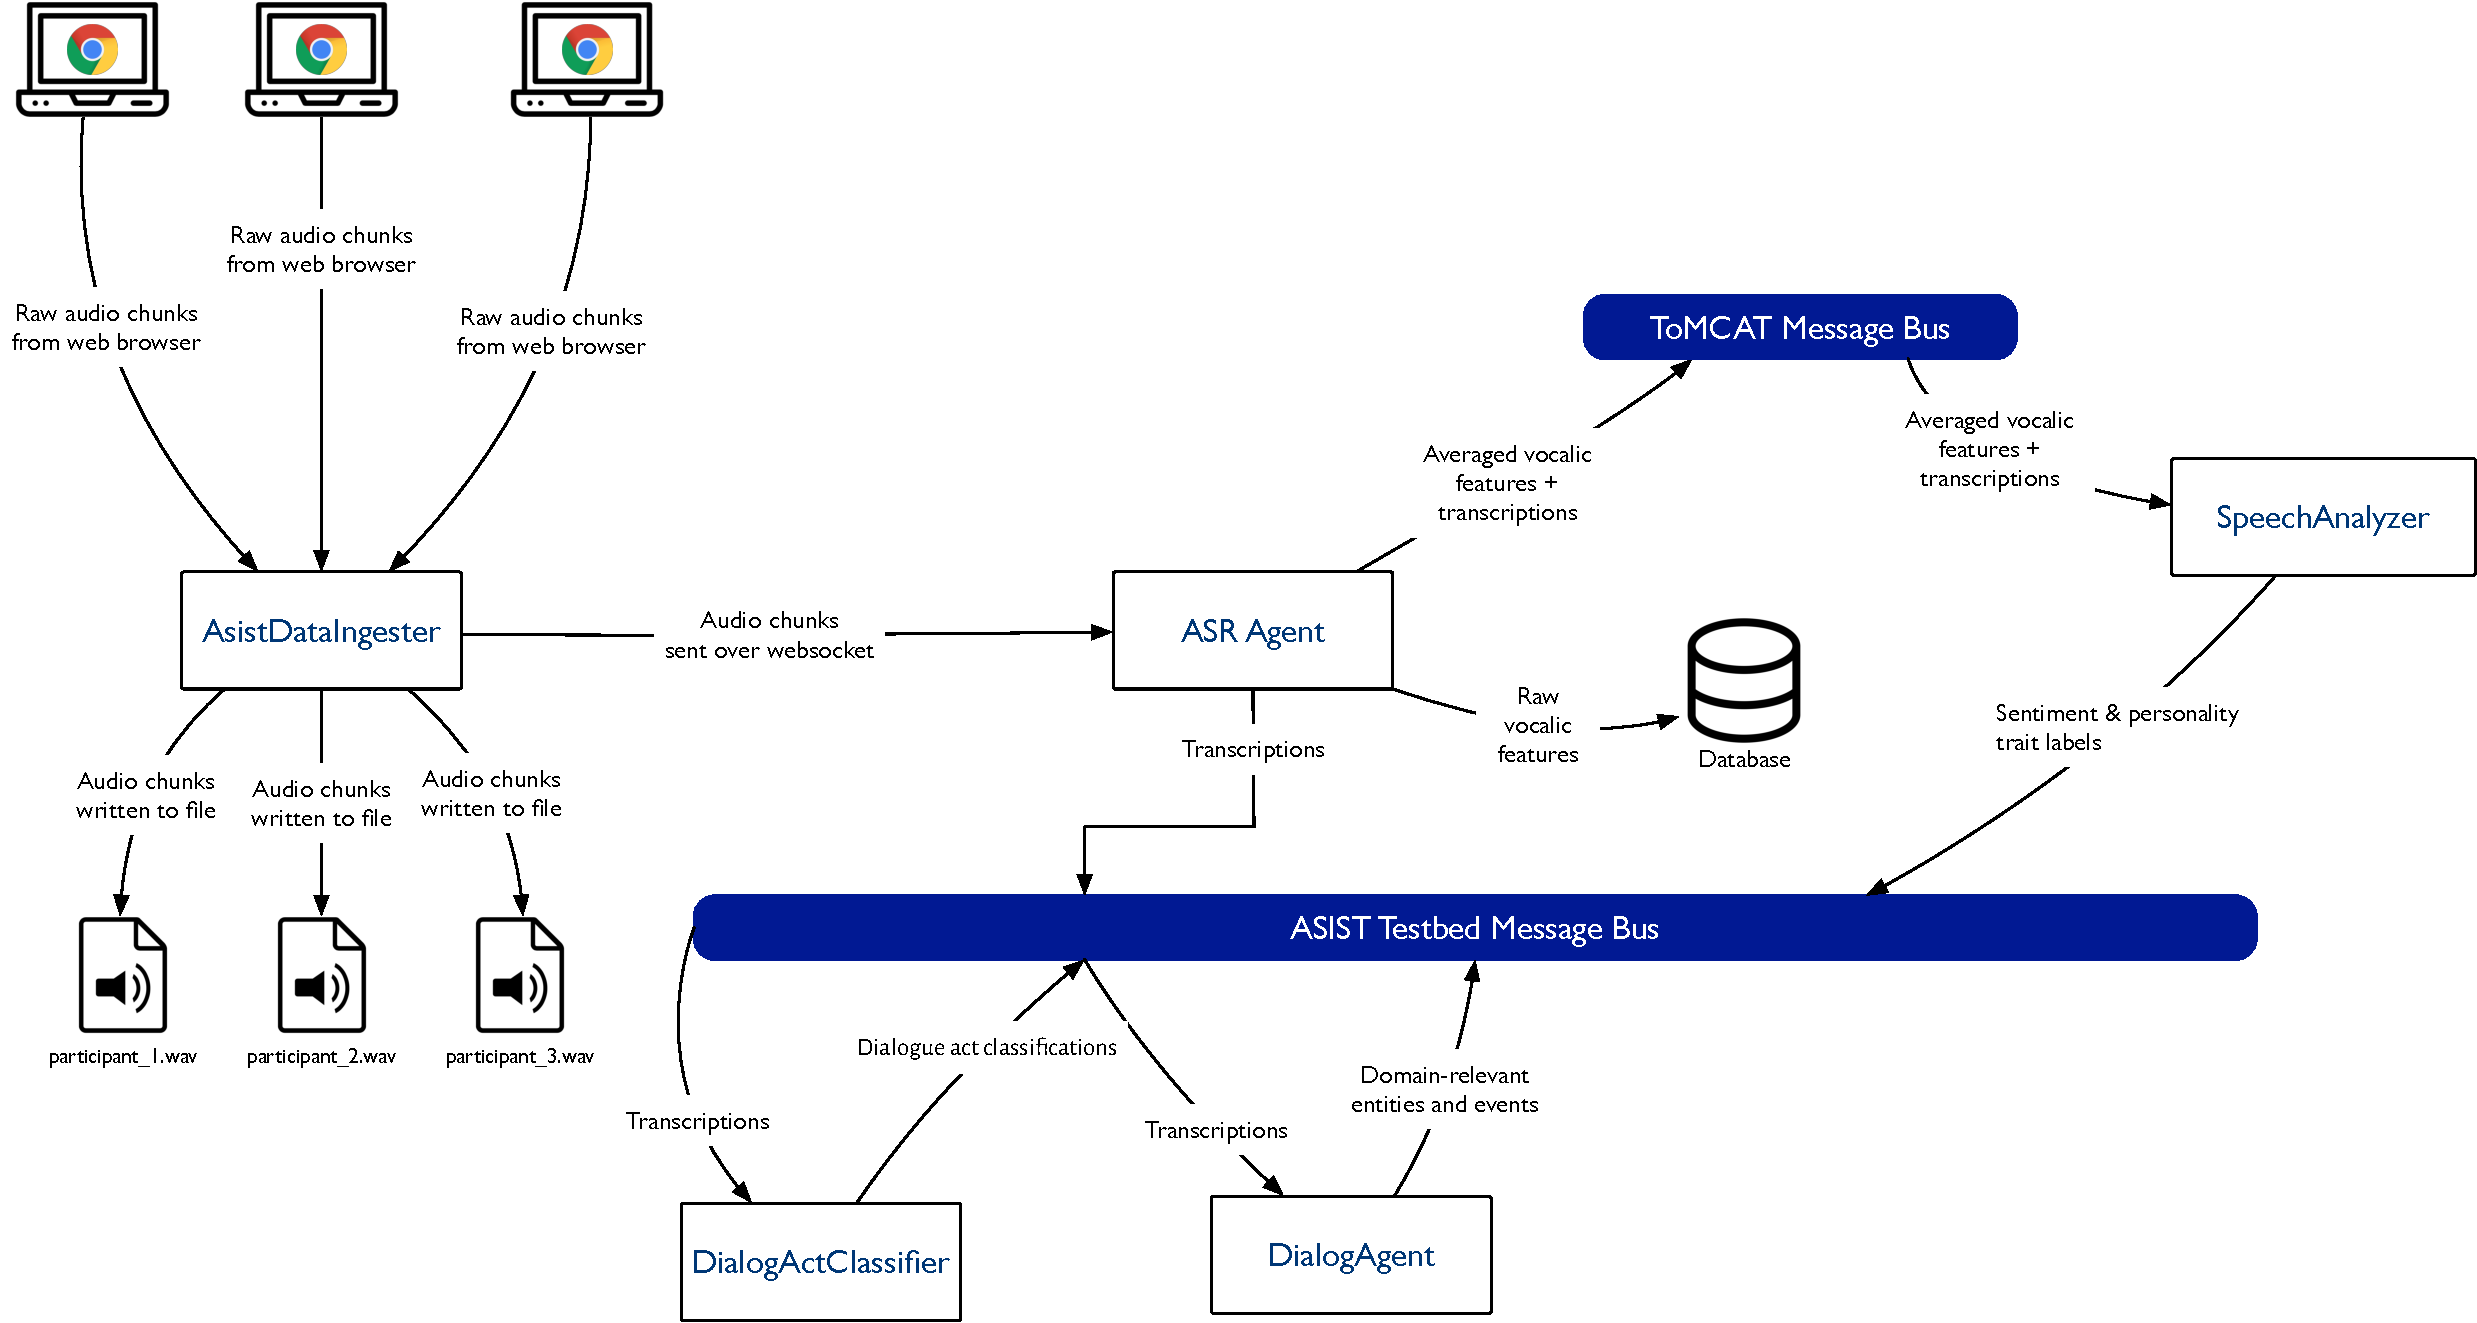
\includegraphics[width=6.5in]{images/nlp_architecture}
    \caption{Architecture of our multi-participant dialogue analysis system.}
    \label{fig:nlp-architecture}
\end{figure}

%Give a brief summary of the preregistrations and how they contribute to the overall architecture.

The component preregistrations in this document span a broad spectrum of
research topics, but work together to form a cohesive suite of ASI
capabilities.

Chapters \ref{ch:rule_based_ie} and \ref{ch:sentiment_analysis} focus on
gleaning information from individual natural language utterances. Chapter
\ref{ch:rule_based_ie} discusses our rule-based system for extracting entities
and events from natural language text, and \autoref{ch:sentiment_analysis}
describes our approach to detecting sentiment and personality traits using both
text and speech information.

In chapters \ref{ch:da_classification} and \ref{ch:clc}, we move
beyond analyzing utterances individually to analyzing them \emph{in context},
that is, we consider windows containing multiple utterances to detect
longer-range phenomena. Chapter \ref{ch:da_classification} uses context to identify
dialogue acts, and \autoref{ch:clc} uses it to automatically detect
closed-loop communication. Chapter \ref{ch:da_classification} also discusses
using multiple modalities (speech and text) to classify dialogue acts.

In \autoref{ch:entrainment}, we discuss our approach to detecting real-time
conversational alignment, or \emph{entrainment} between teammates. In
\autoref{ch:plan_recognition}, we describe our approach to multi-agent plan
recognition. The analyses described in this chapter will be performed offline
for ASIST Study 3, but we expect them to be integrated into online components
for ASIST Study 4 and future experiments.

Finally, we describe our probabilistic modeling approach to machine theory of
mind (MToM) and machine theory of teams (MToT) in \autoref{ch:pgm}, along with
our planned interventions in ASIST Study 3 and their rationale.

\chapter{Probabilistic modeling of team dynamics}
\textbf{Paulo Soares, Kobus Barnard, Emily Butler}
\section{Introduction}
\begin{itemize}
    \item Why is this a useful capability for an AI
        agent? How does it contribute to machine theory of mind/machine theory
        of teams?
    \item What are the existing state of the art approaches to this problem
        (cite relevant papers), and what are their limitations? 
    \item What is our approach, and how will it address those limitations?
\end{itemize}

\section{Approach}
\begin{itemize}
    \item Provide details on our approach, including:
        \begin{itemize}
            \item What data is required for this work? If any of the required
                inputs are present in the table of Study 3 variables in the
                \href{https://docs.google.com/document/d/1GF7VsNF9R95IAaj6mVZUDV2mAX5ok1Bh6Tcm8zDpIkg/edit#heading=h.1ksv4uv}{TA3
                Study 3 preregistration document (table 3)}, please list those
                variables with the standardized verbose variable names in the table.
            \item What interventions will we be testing and why?
        \end{itemize}
\end{itemize}

\section{Evaluation}
\begin{itemize}
    \item How will we evaluate our approach?
\end{itemize}

\chapter{ASR Agent}
\label{ch:asr}
\textbf{Adarsh Pyarelal, Vincent Raymond}

\bigskip

The ASR agent enables the publishing of real-time transcriptions of the
participants' conversations to the message bus. The inputs to the ASR agent are
audio chunks streamed via websockets, with one stream per participant. The
chunks are then sent to the Google Cloud Speech service, which then returns
real-time transcriptions.

The ASR agent then passes along the audio chunks and the transcriptions to the
SpeechAnalyzer via an internal message bus for further downstream processing
(see \autoref{ch:sentiment_analysis}).

While the transcriptions produced by the ASR agent are not perfect, they have
improved significantly compared to the initial release. The improvement can be
attributed to two factors:

\begin{enumerate}
    \item We switched to the premium `video' model offered by Google, which is
        able to handle noisy audio data much better. This change is responsible
        for most of the improvement.
    \item Further improvement was achieved by providing the service with a
        domain-specific list of phrases as hints.
\end{enumerate}

The list of domain-specific phrases we used is given in \autoref{ch:vocab}.

\chapter{Rule-based entity and event extraction}
\label{ch:rule_based_ie}
\textbf{Remo Nitschke}

\section{Introduction}

For humans, verbal and non-verbal communication are indicators that provide
significant insight into social processes. Within the scope of the ASIST
program, team-building and communication within teams is of heightened
interest. We assert that understanding the semantics of verbal communication is
essential to develop a model of human individuals and teams. Our `DialogAgent'
AC is designed with the goal of extracting information from player dialog that
can help build and update a model of players' mental states. The outputs of the
DialogAgent AC are consumed by the ToMCAT ASI (\autoref{ch:pgm}).

Raw natural language data is messy by nature - in order for a machine to reason
about its semantics, it must be processed to extract structured information.
In order to do this, the DialogAgent leverages Odin
\cite{valenzuela-escarcega-etal-2016-odins}, a powerful rule-based information
extraction system developed at UArizona.  While much of modern information
extraction and event extraction is done using neural networks
\cite{Ahmad2021GATEGA, Du2020EventEB}, we opt for a rule-based system for the
following reasons:

\begin{enumerate}

 \item It allows us to be more flexible with our extraction labels. We can
     quickly add or remove labels if we see the need to do so.

 \item It allows for high precision for the labels we are interested in. Rules
     can be crafted to be precise (albeit at the cost of recall).

 \item Rules do not require us to create, maintain, and annotate extensive
     datasets. This is especially pertinent to the ASIST program, with the
     relatively fast cadence of changes to the experimental task and domain,
     along with the concomitant changes to domain-specific vocabulary of
     interest.  It would be near-impossible for us to annotate data and train a
     neural agent on the new vocabulary of a study prior to its actual
     execution and the release of the data from it. 

\end{enumerate}

\section{Approach}

The DialogAgent processes natural language texts from two sources: utterances
spoken by players, and text chats sent using the Minecraft chat
interface\footnote{For ASIST Study 3, participants are discouraged from using
    text chat, but it is not programmatically disallowed - for this reason, we
    still monitor it. Performer teams who use the outputs of the DialogAgent
    should inspect the \texttt{data.participant\_id} key in the DialogAgent
    output messages to make sure that it is not \texttt{Server}, which
correspnods to chat messages sent by the testbed infrastructure rather than
humans.}.

Our rule-based framework extracts \emph{events} from natural language. These
can be either \emph{simple} events, that do not have any arguments, or
\emph{complex} events, that can take other events as arguments. Each event is
associated with a unique span of text and is assigned one or more labels by the
rule that extracts it. The labels we are using are organized into an ontology.
If a rule assigns a label to an event from this ontology, the parents of that
label in the ontology are also assigned as labels for that event.

\section{Evaluation}

We will evaluate via manual evaluation by human annotators. We will hire human
annotators to evaluate a representative chunk of utterances. As the DialogAgent
currently extracts 100+ labels, we have narrow down this selection in order to
avoid overwhelming our annotators.  We will select 20 labels for annotation.
These labels will be selected for two qualities:

\begin{enumerate}

\item Complexity: The DialogAgent labels can be divided in two types. Labels
    which are generated by string-pattern matching and labels which are
    generated by a combination of pattern matching, dependency parsing, and
    tagging. We will call the latter ``complex", as they involve reliance on a
    dependency parse and are more unpredictable due to the fact that they rely
    on multiple conditions to trigger. For this evaluation, ``complex" labels
    are more pertinent, as their accuracy is harder to predict. \footnote{A
        brief explanation as to why ``simple" labels are less interesting.
        Assume a label for players talking about ``victims". This label will be
        generated by a simple pattern matching rule that scans all tokens for a
        regular expression looking something like this: 
               \texttt{/(?i){\textsuperscript{$\wedge$} }victims?\$/}
        .  This pattern will match any and all occurrences of
        ``victim" (plural or singular). The precision and recall of this label
        now depends entirely on the quality of the transcript and on the way
        the players talk about ``victims" (for example, they may use other
        terms as well). This makes this label much more predictable, than one
        that relies on dependency graphs in addition to pattern matching.}

\item High Frequency: The selected label should be sufficiently high in
    frequency to generate a representative amount of data. As our labels are
    often very specific, and thus rare, we will circumvent this issue by
    letting annotators annotate for groupings of labels.\footnote{For example:
    We have five different labels for players ``needing something", such as a
specific item, a specific role, or just help from other players. In order to
lighten the load on annotators, we will subsume these under one label.}

\end{enumerate}

Annotators will receive transcripts of player communications. They will be
asked to annotate the transcripts for the 20 labels we have given them. With
this annotated data, we can write a script that will counter-check the
DialogAgent extractions against the annotations and calculate a representative
F1 score.



\subsection{Precision Evaluation for the Entire Label-Set}

We will also run a seperate evaluation for precision,\footnote{For reasons of
economy, we restrict this evaluation to precision. Our expert team-members can
judge produced labels for precision at a much higher speed than they can
annotate utterances for labels.} done by team members and hired annotators who
are familiar with our DialogAgent labels.


\subsubsection{Preliminary Precision Evaluation} 
We have done a preliminary evalution of 1700 labels for precision already, and have found that the ``simple" labels are highly precise.
``Simple" labels. In our preliminary evalution, simple labels yielded between 91-100\% precision.\footnote{This is for labels that had more than 20 entries in our evaluation}
``Complex" labels are found to yield between 75-94\% precision.\footnote{This is for labels that had more than 10 entries in our evaluation}

\subsection{Potential Evaluation Problems}

By subsuming multiple labels under one label for the general evaluation, we run
the risk of having no way of discerning if one label in a group is a
particularly weak performer. For example, assume we have five different labels
for types of questions. Assume we subsume them under one generic ``Question"
label for this evaluation. After the annotations are done, we calculate an F1
score for this new label. If one of the five labels was a weak performer (for
example, .3 F1), but the others performed well, then the overall F1 score for
this label will mask this fact. 

In order to combat this problem, we will run an evaluation for precision over
the entire label set, as described in the previous subsection. Unfortunately,
we will not be able to generate recall for the entire label set, as this
process is simply too costly for 100+ labels.

\chapter{Sentiment analysis and personality trait detection}
\textbf{John Culnan}
\section{Introduction}
\begin{itemize}
    \item Why is this a useful capability for an AI
        agent? How does it contribute to machine theory of mind/machine theory
        of teams?
    \item What are the existing state of the art approaches to this problem
        (cite relevant papers including \textcite{culnan-etal-2021-ire}), and
        what are their limitations? 
    \item What is our approach, and how will it address those limitations?
\end{itemize}

\section{Approach}
\begin{itemize}
    \item Provide details on our approach, including:
        \begin{itemize}
            \item What data is required for this work? If any of the required
                inputs are present in the table of Study 3 variables in the
                \href{https://docs.google.com/document/d/1GF7VsNF9R95IAaj6mVZUDV2mAX5ok1Bh6Tcm8zDpIkg/edit#heading=h.1ksv4uv}{TA3
                Study 3 preregistration document (table 3)}, please list those
                variables with the standardized verbose variable names in the table.
        \end{itemize}
\end{itemize}

\section{Evaluation}
\begin{itemize}
    \item How will we evaluate our approach?
\end{itemize}

\chapter{Closed-loop communication detection}
\label{ch:clc}
\textbf{Yuwei Wang}

\section{Introduction}

\section{Approach}

We are going to build a rule-based dialogue agent to detect Closed-loop communication events and test the agent using the TA3 dataset.
The existing ToMCAT dialogue system is currently able to analyze spoken
conversations in real-time, to extract entities and events of interest with a
powerful rule-based framework \citep{valenzuela-escarcega-etal-2016-odins}, classify
dialogue acts, and detect sentiment. To extend this system and detect
closed-loop communication, we are going to create a separate worker and detect
the relevant labels based on the three phases of closed-loop communication
within several speech turns, namely, the call-out, check-back, and
closing-the-loop phases \citep{Hargestam.ea:2013}. For example, we can
navigate the call-out phase with Odin labels like ``HelpRequest", and then look
for the ``Move" label in the next 5 speech turns, if we can detect this
check-back phase, keep on looking for additional Closed-loop phase with an
``Acknowledge" label, and return a ``CallOut-CheckBack-Close" extraction. If the
Closed-loop phase is not detected at all, a “CallOut-CheckBack” extraction can
be returned. If both phase 2 and phase 3 are not detected, exit the detecting
loop after 5 steps from the call-out phase and return ``OpenLoop" extraction.

We will firstly implement this agent with a small set of test data, extracted
from the TA3 dataset, and then evaluate the performance of this agent for its
precision, recall, and F1 score, and then explore whether data-driven methods
could improve the score of its performance.

\section{Evaluation}

The agent of the Closed-loop communication detector will be evaluated with a
subset from the TA3 transcripts. Human annotators will be trained to detect the
3 phases of closed-loop communication, and whether the loop is closed or not.
The interrater reliability of the annotators will be measured using Cohen’s
kappa. When the percentage of agreement between annotators reaches 80\%, and K
> .70, annotators could start work on the formal annotation of the data. The
precision, recall, and F1 score will be used to evaluate the performance of our
primary closed-loop communication agent. When improvement on the agent applied,
we can further compare the performance of our primary rule-based model with the
improved model of rule-based and data-driven combined.

\chapter{Dialogue act classification}
\label{ch:da_classification}
\textbf{Ruihong Huang, Ayesha Qamar, Messal}

\section{Introduction}

In the Theory of Mind-based Cognitive Architecture for Teams (ToMCAT) project,
we are working on building an AI agent that will assist the players by taking
their speech and facial expressions as input. Speech being a core part of the
inputs, the agents will need to be capable of natural language understanding to
process the conversations to make informed and prompt decisions. Identifying
Dialog Acts (DA) is one of the primary aspects of natural language
understanding. dialog Act (DA) can be identified as a method of defining the
semantic content and communicative function of a single utterance of dialog
\citep{Searle:1969}. Examples include request, question, acknowledgment etc.
Dialog acts can provide important information about the user dialog turns and
set of possible system actions, and the frequencies and patterns of DAs spoken
by different speakers could also potentially indicate the roles they play such
as leader, follower etc., Thus, it is a useful capability for this AI agent and
many conversational agents in general.

Acknowledging the importance of DA classification in natural language
understanding, extensive research has been conducted on DA classification.
These research works have taken different approaches in terms of dataset,
machine learning model and input to the models. The most popular datasets that
are being used are Switchboard Corpus (SwDA) and ICSI Meeting Recorder Dialog
Act Corpus (MRDA). Most of the approaches use textual utterances from dialog
transcripts as input to the model. Statistical machine learning models such as
Support Vector Machines (SVMs) \citep{Henderson.ea:2012}, Hidden Markov Models
(HMMs) \citep{Stolcke.ea:2000}, Conditional Random Fields (CRFs)
\citep{Zimmermann:2009} are employed for identifying DAs. Deep learning models
are also gaining popularity in DA classification. \citet{Liu.ea:2017} presented
both CNN models and hierarchical CNN+CNN and CNN+RNN models to classify dialog
acts and showed that RNN/Bi-LSTM on top of CNN model performs better than other
models in consideration. \citet{Shen.ea:2016} presented that Neural Attention
Model with context information performed well on the SwDA dataset.
\citet{Raheja.ea:2019} achieved state-of-the-art result using context-aware
self-attention model on MRDA corpus. Another approach for DA classification is
incorporating both lexical and acoustic features. \citet{Ortega.ea:2018} showed
that their Lexico-Acoustic neural network models can outperform the similar
models taking only lexical information as input.

Even though these approaches provide excellent results on DA classification,
they lack in various aspects. First of all, most of these models require clean
transcripts as input. Achieving clean transcripts requires manual annotation,
which is both time consuming and costly. As a result, DA classification in real
time is not possible. Another limitation is the lack of explicit addressing to
multiparty dialogs where mechanisms to incorporate speaker identification and
determining the discourse structure is also crucial. Apart from these
limitations, these approaches often use only 5 types of high level tags for DA
classification, which do not entirely explain the DA under question. It is
necessary to have both general and specific tags to completely understand a DA.

We are going to develop a Deep neural network based DA classifier to process
the input utterances in real time which is more aligned with the main goal of
the project that is building an AI agent to be an effective teammate of a
Minecraft player. As the players will play online simultaneously, the agent
needs to understand the conversations of the player as the game progresses. For
the agent to be real time, we cannot rely on manual transcription. Instead we
have used a publicly available Automatic Speech Recognizer (ASR), named Google
Cloud Speech API to convert the utterances into text. This provides noisy text
in return which might harm the performance of the DA classifier. To compensate
for this, we will use acoustic features from the raw speech as well.

\section{Approach}
A Bi-LSTM based baseline model is already trained with clean transcripts. The
same model is trained again with the ASR generated transcripts and the
performance dropped significantly due to ASR noise and the highly overlapping
nature of the utterances in the meetings. To overcome this drop we will use a
fusion based audio-language model to leverage both lexical and acoustic
information of the utterances to successfully identify the DAs. In addition,
our approach will capture the threading structure within a dialogue that
involves detecting utterances falling within an adjacency pair (consisting of a
question and an answer utterance, or a request and an acceptance utterance) and
then linking them together. We will aim to eventually jointly learn both the
threading structure and DAs of a dialog in a multitask learning setting since
we expect the two tasks to benefit each other.

Currently we are using a multi-party dialog dataset MRDA
\citep{Shriberg.ea:2004} that consists of 75 meetings each about an hour long,
where each utterance has one (out of 11) general and zero or more (out of 40)
specific tags. Once the experimentation is done, we will use a transfer
learning approach to train and test the model for study-2 data. 

\section{Evaluation}

To evaluate our approach, we will use F1 score as the evaluation metric. For
multiclass classification problems, especially where the classes are highly
imbalanced, F1 score provides more insight than accuracy.  We also intend to
annotate ASIST data for dialog Acts so that the system trained on MRDA can be
finetuned on ASIST.

\chapter{Entrainment detection}
\label{ch:entrainment}

\textbf{Meghavarshini Krishnaswamy, Andrew Wedel, Adam Ussishkin, Cheonkam Jeong} 
\section{Introduction}

    Entrainment (also referred to as `synchronization', `coordination', or `alignment') is the adaption of verbal and non-verbal actions by conversation partners to more closely resemble one another \parencite{borrie2014}. Its role in communication as been described as ``key for supporting important pragmatic aspects of conversation, including taking turns, interaction smoothness, building rapport, fostering social bonds, and maintaining interpersonal relationships''\parencite{borrie2019}. A time-sensitive cooperative task utilizing verbal communication would require participants to optimize their information channel. This makes entrainment a useful metric for assessing the degree of cooperation among teammates, as well as a useful means to assess members' sentiments towards each other, tracking their confidence in the task goals and plans, and identifying team cohesion and bonding over time.

    In speech, entrainment has been observed and analysed using speech rhythm and
    timing, pitch, MFCCs and formant analysis \parencite{reichel2018prosodic,borrie2019syncing}. Speech entrainment occurs in correlation with entrainment at other linguistic levels such as an increase in shared vocabulary and sentence structures \parencite{rahimi2017entrainment}. While entrainment in multi-party conversations has been researched at the lexical-level and sentence-level, speech entrainment has mostly been restricted to two-party conversations. Work on speech entrainment is further limited by the practical difficulties in identifying speech similarity due to the process of entrainment from similarities from physical factors such as people having similar vocal characteristics, or sharing the same speech channel \parencite{nasir2020}.

    Recent research on vocal entrainment has shifted from regression-based analysis to encoding-based neural networks for a few reasons: to model the non-linear relationship between vocalic features, to capture the complexity and diversity of both entrainment and disentrainment, and to train the model on information relevant to entrainment, while ignoring other factors that cause similarity (such as speaker characteristics and features related to the speech recording channel)\parencite{nasir2020}.


\section{Approach}
    The main assumption for automated entrainment detection is that for a given set of speakers and utterances in a discourse, if entrainment takes place, it is located between two neighbouring utterances from different speakers, while utterances from different time points will not show entrainment. So, the model needs to correctly identify neighbouring pairs of utterances, while ignoring similarities pertaining to speaker and channel characteristics (since they are not a function of entrainment). For a multi-party conversation setting, the model also needs to tell the difference between a pair of entrained utterances, a pair of utterances from the same speaker, and utterances from different speakers that are not neighbours.

    Our approach involves training an replicating the feed-forward encoder model and i-vector modelling for entrainment detection proposed and designed by \citeauthor{nasir2020}. This model assess triplets of utterances for each speaker arranged as follows: an utterance by a given speaker, the utterance succeeding it spoken by a different speaker (positive match for entrainment), and an utterance from a different location in the discourse uttered by the given speaker (negative match for entrainment). In the training process, positive weights are assigned to entrainment characteristics, while speaker and channel characteristics are assigned negative weights. We thus have a classification task in which for a given pair of utterances, we ask if one is the entrainment pair of the other or not.

    \begin{figure}
    \begin{sidecaption}{Representation of the triplet model proposed by \citeauthor{nasir2020}[Pg17]. Here, ``Speaker 1 (anchor)'' and `Speaker 2 (positive)' refer to the site of entrainment, while `negative' refers to a non-entrainment utterance}
    \centering
    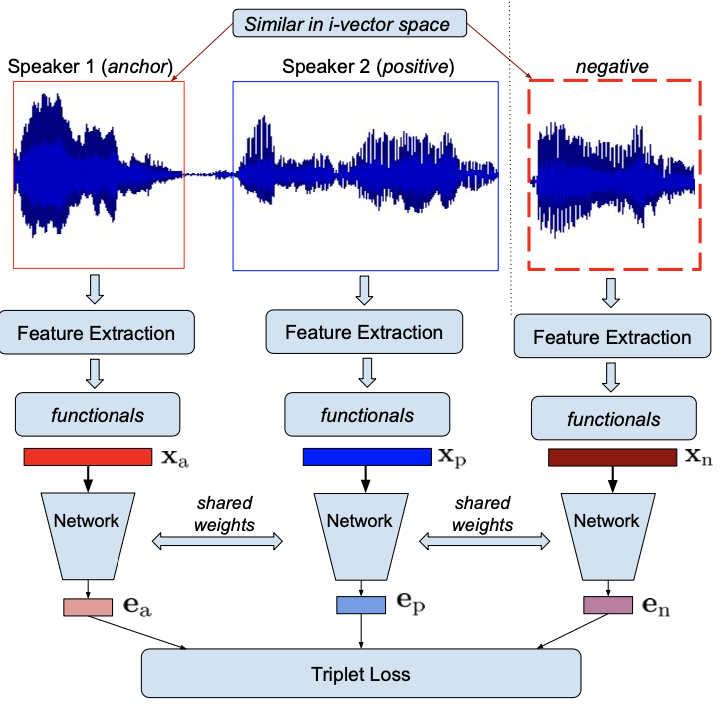
\includegraphics[width=0.6\textwidth]{images/triplet-model.png}
    \label{fig:sentiment_model_schematics}
    \end{sidecaption}
    \end{figure}

    We will utilize the following data and labels from Study-3-
            \begin{itemize}               
                   \item Audio recording
                    Transcript
                   \item Participant demographic information
                   \item Self-evaluation
                   \item MinecraftEntity\_Observation\_Asr\_Speechanalyzer
                   \item MinecraftEntity\_Observation\_Audio\_Speechanalyzer
                   \item MinecraftEntity\_Event\_Dialogue\_Event\_Dialogagent
            \end{itemize}
        % \item Our objectives (in decreasing order of priority):
        %     \begin{itemize} 
        %         \item Build a working statistical model for assessing entrainment while utilizing the vocalic features extracted by the ToMCAT-speechanalyzer system.         
        %         \item Train an encoding-based model using the methodology outlined in \textcite{nasir2020} for a simple classification task that identifies entrainment and directionality in a given conversation.
        %         \item Assess if the current Speechanalyzer system is set up to study entrainment trends as a time series. 
        %     \end{itemize} 

\section{Evaluation}

    Assessing entrainment involves calculating a similarity (or dissimilarity) measure between two utterances from the entrainment category, and to observe if this metric of similarity increases or decreases as the speakers continue communicating. For this objective, accuracy scores for the classification task outlined above will be used to measure the performance of the entrainment detector. Because ASIST-ToMCAT is a multi-party conversation, we will examine the process of setting up new baselines for entrainment detection that can account for differences in team dynamics, reflected in how much each speaker talks, and how much other speakers respond to them.  

    We will also explore methods to evaluate two types of entrainment:

    \begin{itemize}
        \item Localized entrainment: Are there observable similarities between utterances by different speakers that occurred next to each other than utterances at different points in time?
        \item Global entrainment: after a given period of objective-oriented speech, is the speech from the conversation aligned more closely? 
    \end{itemize}

    In order to account for ASR errors in the automatically generated transcripts, we will create a corpus of human-generated gold transcriptions. From this corpus, a subsection of the data will be used to identify utterances separated by 50ms pauses; in order to assess any differences in performances due to ASR issues. A manual evaluation of the speech data will also be conducted to examine other environmental noise, so as to account for qualitative differences between the recording conditions of the pristine training data and the real-time ToMCAT speech data. 

   \section{Other Qualitative Assessments}

   Since speech entrainment in conversational setups is a feature of speaker bonding and closeness, it is useful to assess if it co-occurs with positive emotions in spoken statements, lower stress, and higher confidence in the plan and team actions in a co-operative goal-oriented setting. We will utilise the human-generated gold transcriptions as well as manual annotations for emotion and dialogue acts to qualitatively assess if entrainment co-occurs with positive emotions and the acts of sharing information, as well as the relationship between global entrainment and levels of stress and uncertainty. We will also examine if the directionality of entrainment (towards or away from any of the participants) is affected by members' personality or socio-cultural differences, in order to account for natural differences known to impact conversation styles.


\chapter{Online multi-agent plan recognition}
\label{ch:plan_recognition}
\textbf{Loren Champlin, Salena Ashton, Liang Zhang, Clayton Morrison}

\section{Introduction}

Plan recognition is the ability to understand and recognize logical structures
and patterns within a sequence of observed behavior. Developing this capability
for our AI agent would allow it to infer the latent plan structures,
strategies, and goals (i.e., `plan explanations') of not only individual human
agents but a team of agents as well. Producing these plan explanations
contributes to the logical belief structures that the AI agent must maintain as
part of its theory of mind and theory of teams
\citep{Tambe_1997,Baker_Tenenbaum_2014}. Furthermore, an AI agent could use
these inferred plan explanations to predict the teams' subsequent actions and
to help develop potential interventions for increasing team performance. Our AI
agent must recognize the conjoined plan explanations of multiple agents given
our team search and rescue setting and demonstrate this capability online
(i.e., as the team carries out their mission). While a highly sparse topic,
there are a few existing "state of the art" approaches for online Multi-Agent
Plan Recognition (MAPR). 

The most recent online MAPR approach by \citet{Argenta_Doyle_2017} uses an automated planner to produce feasible plan explanations by simulating potential sets of parameters, conditions, and plan structures needed to generate the observed behavior. Approaches of this type are known as \textit{plan recognition as planning approaches} \citep{Ramirez_Geffner_2009,Van-Horenbeke_Peer_2021}. The use of an automated planner requires constructing a symbolic representation of the problem domain in which MAPR is to be deployed, known as knowledge engineering. Plan recognition as planning approaches are typically highly expressive and are capable of solving plan recognition problems that involve high levels of logical reasoning. However, this high expressivity usually comes at the cost of the high computational complexity required by the automated planner \citep{Van-Horenbeke_Peer_2021}. \citet{Argenta_Doyle_2017} attempt to overcome this challenge by making several strict simplifying assumptions about their problem domain. Although, these assumptions reduce the computational complexity at the cost of expressivity (i.e., it limits the type of problems their approach can solve). Another limitation is that \citet{Argenta_Doyle_2017} only consider ``flat" knowledge representations, rendering their approach incapable of inferring more than just the end-goals that the agents are trying to achieve. However, human behavior tends to exhibit hierarchical structures or patterns such that simple actions are combined to produce more complex actions. In terms of having a complete theory of mind and theory of teams, an AI agent needs to understand how actions relate to each other at different levels of granularity and complexity, not just how they relate to the agents' end-goals. 

Our proposed method for online MAPR is also a \textit{plan recognition as planning} approach. Rather than make assumptions that limit the problems our approach can solve, we try to overcome the challenges of computational complexity by developing a highly efficient automated planning algorithm specialized towards doing online MAPR. Our automated planning algorithm combines the well-known Simple Hierarchical Ordered Planner (SHOP2) proposed by \citet{Nau_2003} and the Monte Carlos Tree Search (MCTS) single-agent plan recognition algorithm proposed by \citet{Kantharaju_Ontanon_Geib_2019}. We also draw heavy inspiration from known parsing algorithms for Probabilistic Context-Free Grammars (PCFG) \citep{Collins_2011}. As suggested by its partial adaption of the SHOP2 algorithm, our approach assumes that the agents' actions relate through a set of hierarchical structures or what is known as a hierarchical task network (HTN) \citep{Nau_2003,Russell_Norvig_2021}. As such, our approach produces the most likely task hierarchy, which is an instance of a HTN under specific initial conditions. These task hierarchies represent how actions relate to each other at different levels of granularity of complexity by showing how high-level actions (also known as compound tasks) can be decomposed into low-level actions. 

\section{Approach}
In a HTN domain representation, compound tasks are high-level actions that are
composed of lower-level actions. These lower-level actions may be compound task
themselves that need to be further decomposed or non-decomposable actions,
which are sometimes referred to as primitive tasks or just actions
\citep{Russell_Norvig_2021}. Depending on how abstractly a compound task is
defined, there may be multiple sets of lower-level actions that could be
combined to create the same compound task. These different sets of actions are
known as ``methods", since they are different ways of decomposing the compound
task \citep{Russell_Norvig_2021}. Additionally, methods typically have
preconditions, which are specific conditions that must be satisfied by the
current state of the problem domain for that method to be used for task
decomposition. If a methods preconditions are satisfied, then that method is
said to be applicable \citep{Russell_Norvig_2021}. \autoref{fig:pr1} further illustrates the concepts of compound tasks, actions, methods, and task decomposition. In the illustration, both methods could applicable or only one of them could be applicable given the current state of the problem domain. In the former case, an automated planner must choose one of the methods for decomposition, leading to two different possible plans. Further details on HTN planning processes can be found in the automated planning literature. (e.g., the SHOP2 paper by \citet{Nau_2003}). 

\begin{figure}
    \centering
    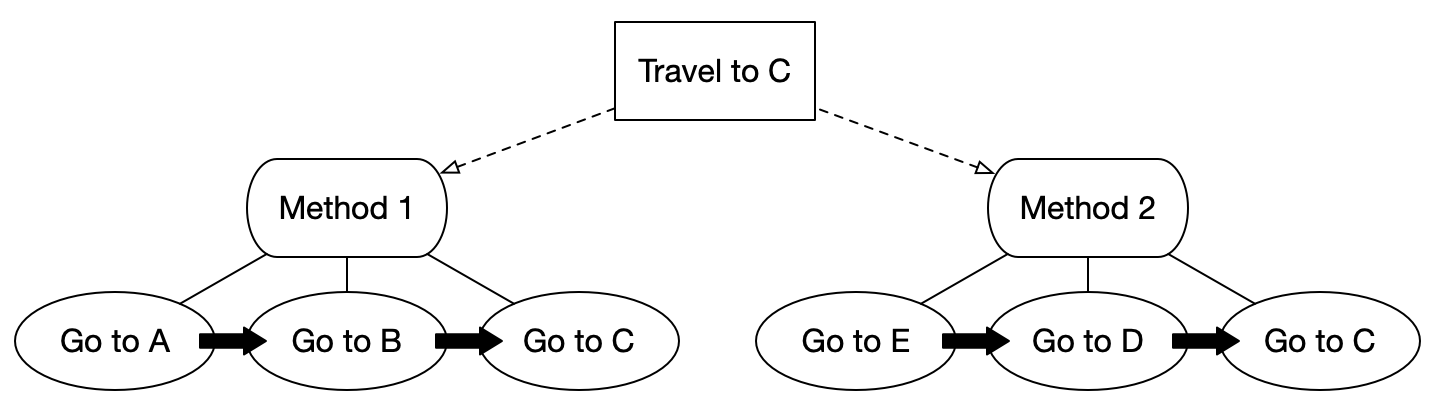
\includegraphics[width=\textwidth]{../images/htn_concepts}
    \caption{The compound task \textit{Travel to C} is shown to have two different methods for accomplishing the same task.} 
    \label{fig:pr1}
\end{figure}

Our approach uses a HTN domain representation and an automated HTN planner to
model the logical reasoning and decision-making process of a team of human
agents. Compound tasks and methods are engineered in such a way as to represent
the latent decisions that agents must make to complete their mission. From a
generative perspective, these latent decisions are then what leads to the
actions we observe from the human agents. With this concept in mind, we can
have an automated planner generate a plan that matches the observed actions
while recording the methods and task decompositions involved. As suggested in
the introduction, this record is produced in the form of a task hierarchy which
shows how compound task can be decomposed into the actions we observe. These
task hierarchies are the plan explanations that give insight on the
relationship between actions and the decision-making process of the agents.
\autoref{fig:pr2} illustrates the general concept of our online MAPR approach.

\begin{figure}
    \centering
    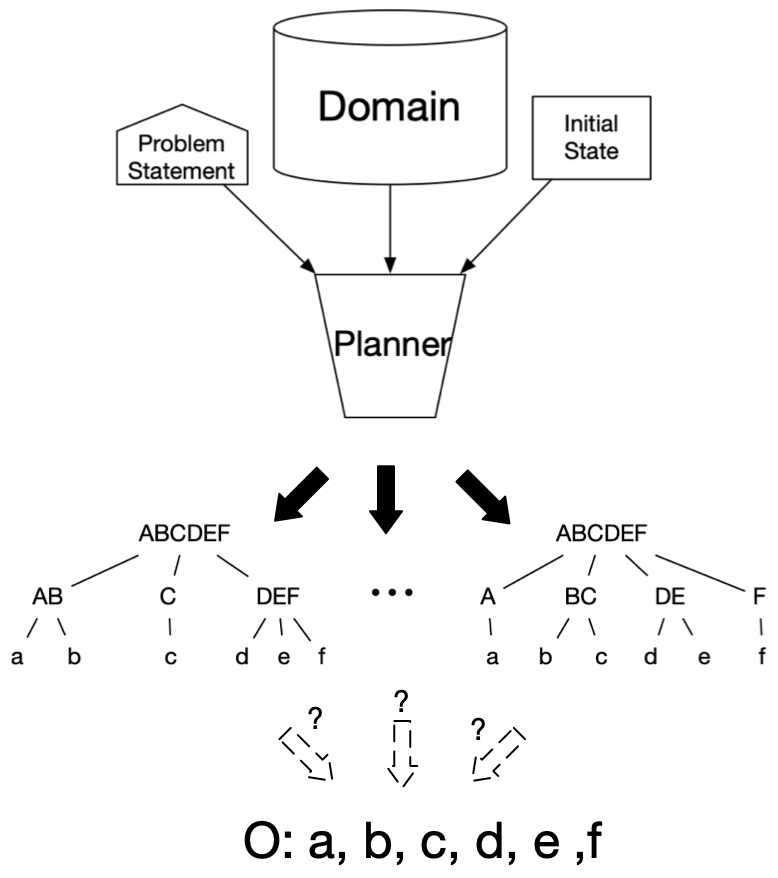
\includegraphics[width=\textwidth]{../images/pr_as_planning}
    \caption{In this illustration compound task are represented as groups of upper-case letters and actions are singular lower-case letters. Multiple potential task hierarchies can be generated for the same observed plan.} 
    \label{fig:pr2}
\end{figure}

As seen in  \autoref{fig:pr2}, it is possible that there are multiple plan explanations for same observed actions. However, rather than obtain all potential plan explanations given an observed sequence of actions, our approach should be yielding the most likely plan explanation. With this in mind, our approach assigns a conditional probability $p(m | \bigcap_{n \in M_t} c_n(s), s)$ for a method $m \in M_t$ for a compound task $t$. $c_n(s)$ denotes a function that is 1 if $n \in M_t$ is applicable to $t$ for the current state $s$, and 0 otherwise. The conditional probabilities are then defined as,

\begin{equation} \label{pr_eq:1}
p(m | \bigcap_{n \in M_t} c_n(s), s) = \begin{cases} \alpha  & c_m(s) = 1 \\ 0 & c_m(s) = 0 \\ \end{cases}
\end{equation}

\begin{equation}  \label{pr_eq:2}
\sum_{m \in M_t} p(m | \bigcap_{n \in M_t} c_n(s), s) = 1
\end{equation}

The value denoted by $\alpha$ in (\ref{pr_eq:1}) of each conditional probability must be predefined. As part of our approach we have formulated a training algorithm for learning these conditional probabilities, however that training algorithm is not detailed here. 

As suggested, an automated planner uses the methods defined in a HTN domain representation to decompose a compound task or set of compound tasks into a plan. This derivation of a plan is an analogous process to deriving a sentence from a PCFG. A PCFG contains a vocabulary of both non-terminal symbols and terminal symbols, as well as a set of derivation rules for replacing non-terminal symbols with a sequence of both non-terminal and terminal symbols \citep{Collins_2011}. Given an initial non-terminal symbol and applying rules successively eventually yields a sequence of only terminal symbols (i.e., a sentence) \citep{Collins_2011}. Similar to the methods of our HTN domain representation, each derivation rule is assigned a probability. Thus, given a specific derivation of a sentence (i.e., a specific set of derivations rules used), the probability of that derivation is the product of the probabilities of each rule used \citep{Collins_2011}. Given the similarities, we define the probability of a specific task hierarchy for a given plan in the same way. We denote $m_t$ as the applicable method chosen to decompose task $t \in \tau_\pi$, where $\tau_\pi$ is a set of tasks representing some task hierarchy used to generate a plan $\pi$. Using (\ref{pr_eq:1}), we have that,

\begin{equation} \label{pr_eq:3}
p(\tau_\pi) = \prod_{t \in \tau_\pi} p(m_t | \bigcap_{n \in M_t} c_n(s_t), s_t) 
\end{equation}

$s_t$ is current state prior to the decomposition of task $t$. Since our approach is for online MAPR, we want our plan explanations to consist of a partial task hierarchy that shows how the agents' latent decisions generates their plans up to the current time step. We denote the agents' observed partial plan (i.e., their observed sequence of actions up to some current time step) as $\pi^*$. We then simply replace $\pi$ in (\ref{pr_eq:3}) with $\pi^*$ to get,

\begin{equation} \label{pr_eq:4}
p(\tau_{\pi^*}) = \prod_{t \in \tau_{\pi^*}} p(m_t | \bigcap_{n \in M_t} c_n(s_t), s_t) 
\end{equation}

Using (\ref{pr_eq:4}), the objective of our approach is then to compute 

\begin{equation} \label{pr_eq:5}
\hat{\tau}_{\pi^*} = \argmax_{\tau_{\pi^*} \in T_{\pi^*}} p(\tau_{\pi^*})
\end{equation}

In (\ref{pr_eq:5}), $T_{\pi^*}$ denotes the set of all partial task hierarchies that match the observed partial plan $\pi^*$.

SHOP2 uses a depth first search (DFS) algorithm to generate plans and as such we could modify it to generate $T_{\pi^*}$ and then compute $\hat{\tau}_{\pi^*}$ by comparing $p(\tau_{\pi^*})$ for all $\tau_{\pi^*} \in T_{\pi^*}$ \citep{Nau_2003}. This is however an extremely computationally complex procedure and not a feasible method, especially for online MAPR where we would need to run this same computation many times. In general, using any automated planning algorithm to generate $T_{\pi^*}$ is not feasible. 

We argue that reasonable method would be to instead sample partial task hierarchies from $T_{\pi^*}$ and estimate $\hat{\tau}_{\pi^*}$ instead, this estimate being denoted $\bar{\tau}_{\pi^*}$. \citet{Kantharaju_Ontanon_Geib_2019} had come to this same conclusion in their development of an approach to do single-agent plan recognition using a domain representation based on Combinatory Categorical Grammars (CCGs). As mentioned in the introduction, they use a MCTS algorithm to sample the space of plans and find a reasonable estimate of the most likely plan explanation for an observed plan, reducing the computational complexity of their approach significantly. Using a similar concept, we modified the SHOP2 algorithm to use a MCTS algorithm as opposed to DFS. Although we will not go into full details here, MCTS samples solutions from the search space, which in our case are partial plan hierarchies matching the agents' observed partial plans. The search algorithm uses each sample to compute statistics about the search space that inform it where ``good" areas of the search space are according to some utility function \citep{Browne_Powley_Whitehouse_Lucas_Cowling_Rohlfshagen_Tavener_Perez_Samothrakis_Colton_2012,Kantharaju_Ontanon_Geib_2019}.In our case, our utility function is $p(\tau_{\pi^*})$, which the algorithm attempts to maximize. MCTS balances its search between completely unexplored areas and areas of the search space that have yielded good results before \citep{Browne_Powley_Whitehouse_Lucas_Cowling_Rohlfshagen_Tavener_Perez_Samothrakis_Colton_2012,Kantharaju_Ontanon_Geib_2019}. Given enough search time, our MCTS algorithm will eventually compute $\hat{\tau}_{\pi^*}$, although the needed search time would be roughly equivalent to what SHOP2 would need to do the same task. Therefore we must limit the search time allowed and have our algorithm return the best $\tau_{\pi^*}$ it can find under a predefined search time, which is our estimate $\bar{\tau}_{\pi^*}$. There is a high chance that $\bar{\tau}_{\pi^*}$ may only be a local optima, but it is likely to be a sufficiently probable plan explanation given a reasonable amount of search time. 

In terms of the Study 3 data, our approach heavily utilizes the json mission event messages coming from the message bus during the Search and Rescue mission trials. These messages are primarily used as the observations for our plan recognition algorithm, but are also used along with the video of the trials as source material for knowledge engineering our HTN domain representation. We also use the messages in our training algorithm to learn the conditional probabilities as defined in \ref{pr_eq:1} and \ref{pr_eq:2}. The specific input variables that we use in our approach from the message bus are as followed, 

\begin{itemize}
\item MinecraftEntity\_Event\_Triage\_Simulator
\item MinecraftEntity\_Event\_Roleselected\_Simulator
\item MinecraftEntity\_Event\_Proximityvictiminteraction\_Simulator
\item MinecraftEntity\_Event\_Playerfrozenstatechange\_Simulator
\item MinecraftEntity\_Event\_Tooldepleted\_Simulator
\item MinecraftEntity\_Event\_Markerplaced\_Simulator
\item MinecraftEntity\_Event\_Markerremoved\_Simulator
\item MinecraftEntity\_Event\_Markerdestroyed\_Simulator
\item MinecraftEntity\_Event\_Victimpickedup\_Simulator
\item MinecraftEntity\_Event\_Victimplaced\_Simulator
\item MinecraftEntity\_Event\_Rubbleplaced\_Simulator
\item MinecraftEntity\_Event\_Rubbledestroyed\_Simulator
\item MinecraftEntity\_Event\_Victimnolongersafe\_Simulator
\item MinecraftEntity\_Event\_Missionstate\_Simulator
\item MinecraftEntity\_Event\_Location\_Locationmonitor
\item MinecraftEntity\_Event\_Victimsexpired\_Simulator
\item MinecraftEntity\_Observation\_State\_Simulator
\item MinecraftEntity\_Observation\_Fov\_Fovtool
\item MinecraftEntity\_Event\_Dialogue\_Event\_Dialogagent
\end{itemize}

\section{Evaluation}
Since it would be extremely difficult to objectively confirm a teams latent decision process used for a mission trial, we have devised an alternative evaluation method for testing the performance of our online MAPR approach. The algorithm described in our approach section, can be reconfigured to project forward in time past the agents' observed partial plan, effectively allowing it to predict their most probable next actions using $\bar{\tau}_{\pi^*}$ as a reference point for the agents' latent decision-making process. We reason that the closer $\bar{\tau}_{\pi^*}$ is to the true value, the more accurate the action prediction will be. Using this concept, we can indirectly measure how well our approach works by measuring how accurate the action predictions are given $\bar{\tau}_{\pi^*}$.

While our algorithm could technically project forward to the end of a team's mission trial, we expect the prediction accuracy to increasingly diminish as the gap between the end of the projected plan and the observed partial plan increases. Instead we evaluate our algorithms performance by having it use $\bar{\tau}_{\pi^*}$ to predict only the next few actions. Given an observed plan from a completed mission trial, we can simulate having a teams' observed partial plan at a set time points in their mission. At these set time points, we can run our online MAPR algorithm and then have our planner predict the next few actions, and compare these predicted actions against the teams' true actions. 

We will compute two different types of accuracy measures, the action allocation accuracy and the action sequence accuracy, which are accuracy measures used in other MAPR literature \citep{Kim_Chacha_Shah_2015}. The action allocation accuracy is the ratio of how many predicted actions were correct out of the number of actions predicted \citep{Kim_Chacha_Shah_2015}. The action sequence accuracy is computed by first dividing the correctly predicted actions into pairs and then counting how many pairs are in the correct order (regardless of what actions they are predicted to have between them). This count is divided by what the count would be if all pairs were correctly ordered \citep{Kim_Chacha_Shah_2015}. The average action allocation and average action sequence accuracy over all trials will be computed for each prediction point, as well as average accuracy measures over all prediction points over all trials. 

We will also measure the rate at which our prediction accuracies decrease as we increase the number of actions predicted. This can be done by picking a singular prediction point for each trial and measuring the action allocation accuracy and action sequence accuracy as we increase the number of actions predicted. Increases in te number of actions predicted will be done at set intervals (e.g., 2 actions, 4 actions, 6 actions, etc).  Average accuracies will then be computed for each interval over all trials. 

\chapter{Question-Asking and Plan Inference}
\label{ch:question_plan}
\textbf{Salena Torres Ashton, Stephen Kim, Loren Rieffer-Champlin, Liang Zhang,
Adarsh Pyarelal, Clayton Morrison}
%% Start on line 115

\section{Summer 2022 Introduction}
\subsection{Significance of Question-Asking in SAR Scenarios}
When we share information\footnote{The Introduction and Evaluation sections of this chapter have been significantly rewritten. To maintain transparency, the Approach section has remained as written in the preregistration. As a consequence, some redundancy may be found between sections.}, clarify ambiguity, or optimize instruction execution, we often do so through question-asking and question-answering. This mode of communication often reflects our intention, strengthens relationships, increases productivity, reduces risk, and creates an equitable environment \citet{rothe_lake_gureckis_2018} and \citet{alaimi_2020} between dialog partners. In the SAR scenario implemented for ASIST Study 3, teams of human players engage in cooperative behavior to search for, stabilize, and rescue victims within a collapsed building. As human players verbalize plans, make suggestions, or tell each other what to do, they also ask questions that can infer hidden goals or intentions. Question-asking enables teammates to reduce their individual knowledge asymmetry.  

Not understanding a goal or intention can be seen in the designs of artificial intelligence agents that may have been programmed with researcher bias. If that AI agent's purpose is to assist humans in a SAR scenario, the programmer and researcher must check (or augment) their own domain knowledge of SAR communications in order to curb potential bias toward academic best practices regarding the programming of uncertainty, belief and reinforcement learning. Understanding SAR communications facilitates programmers to design a realistic and scalable domain; not doing so, or at least not consulting SAR experts regarding their information-gathering and sharing habits, can result in flawed domains that predict human player and AI agent action at no better than chance. 

Therefore, question-asking and information-sharing is vital in a domain definition of a Search and Rescue scenario (SAR)  as much as it is in real life. The INSARAG marking system\footnote{FEMA has a similar marking but is only used in the United States, whereas INSARAG is used internationally.} is designed to immediately answer the most frequently-asked questions a rescuer will have in an urban SAR disaster: Go or No-Go, number of live victims, number of dead victims, number of unaccounted-for victims, hazards, building floor references, cleared areas of building, and cleared building \citet{insarag_2022}. SAR workers further communicate with each other through radio, sound horns, Morse code, and direct communication with victims and each other.

This registration investigates the gap between question-asking in natural language discourse and player goals through goal inference. In the SAR scenario implemented for ASIST Study 3, teams of human players engage in cooperative behavior to search for, stabilize, and rescue victims within a collapsed building. As human players verbalize plans, make suggestions, or tell each other what to do, they also ask questions that can infer hidden goals or intentions. Using procedural Grounded Theory to annotate video observations of teams who play Minecraft in an urban search and rescue scenario, we then map players' utterances to action and intention. Actions and intentions are then mapped into action and task definitions of the HDDL declarative language\footnote{See previous section, written by Loren Champlin et al for a description of HDDL and our plan recognition development.} The results of this study show that teams who ask more questions at a more consistent rate lead to better team performance than teams who ask fewer questions, ask more how-to questions, or use questions as a polite way to give directions to teammates. The registration concludes with suggestions for further research development regarding the knowledge engineering and representation of tasks, goals, and hidden intentions. While simple human goals may be represented with classical AI planning, we believe that complex goals with constraints or multiple levels of abstraction may be best represented by a \emph{hierarchical task network} (HTN)\ap{Add a definition of HTN here}, which is a tree of possible plans.\footnote{Technically, the plans produced by HTN planners can also be represented with flat lists - however, in this section, we use the term `plan' to refer to the actual `plan tree' that contains the task decompositions
as well, rather than just the plan alone.}

\begin{enumerate}
    \item How do spoken questions reveal another person's plan or intent? 
    \item Can people listen to spoken questions and accurately decide if the other person's plan is sequential or hierarchical? Can the distinction between such structures improve predictive performance for Artificial Social Intelligence (ASI) agent intervention?
\end{enumerate}

Artificial Intelligence (AI), Information Retrieval, and Natural Language Processing yield exciting research into question-\emph{answering}, relevant document retrieval, Theory of Mind (ToM), and human-computer interaction. However, the literature is sparse within the  \emph{intersection} of artificial intelligence, psycho linguistics, indirect speech acts, negative knowledge modeling, ToM, and question-\emph{asking}. Hawkins and Goodman address this sparsity and the trend of past research to focus on the optimization of question-answering, not question-asking \citet{hawkins_goodman_2017}. 

\subsection{Literature}
When we ask questions, we are not seeded with a set of questions or handed a set of 'correct and incorrect' questions. We do not prefer questions with literal, logical answers \citet{rothe_lake_gureckis_2017} and \citet{clark_1979}. However, most research has focused on answer sets or query matching, preference for concise questions and answers. In reality, people ask open-ended questions, sloppy half questions, use questions to politely tell others what to do, and meander in speech without purpose \citet{brown_1980}. We ask questions to express goals. 

Goals reflect a desired endpoint or world state. A goal can be motivated by belief, desire or intent. People ask questions that either express a goal or infer a hidden goal. A question is the interpretation and response of a hidden (or uttered) goal to be discerned
by another person, typically a dialog partner \citet{hawkins_goodman_2017}. Indirect speech acts and question-answer dialog is a form of \emph{information asymmetry}: a questioner has a goal but needs information, while an answerer has information but does not know the questioner’s goal. Missing or contradictory information naturally leads to a knowledge goal and the generation of questions. The person is then motivated to ask a question \citet{alaimi_2020}. 

Intentions demonstrate action choice to reach that goal-- it is reflected in the way a question is to be asked. A questioner believes that the listener’s knowledge base has information that can facilitate the questioner’s goal.  The type of questions then asked will depend on context, social inference, and other signals in a dialog setting. The key is to decouple\footnote{Hawkins and Goodman's 2017 work was limited to epistemological questions and cooperative behavior.} the inferred goal from the explicit meaning of the question \citet{hawkins_goodman_2017}. This redefinition of \emph{What is a Question} enables models to account for context and avoid assumptions. 

Questions can be viewed as a hidden goal or intent, but they can also be viewed as a way to provide or reinforce knowledge \citet{alaimi_2020} and \citet{ray_2001}. Question-askers want the listener to directly understand their goal, or to discern a hidden goal, or both-- then to give appropriate responses (however that appropriate response may be for the context). When question-askers do not receive appropriate answers from listeners, both dialog partners use conversational implicature and politeness to reach a mutual understanding. They will minimize potential transaction and opportunity costs in conversation to reach mutual understanding.  




\section{Approach}

We assume that questions have hidden goals and infer plans. As teams ask more
questions of each other, human team ToM converges toward cooperative behavior.
We will investigate whether question-asking is associated with \emph{team
planning}, defined as a set of goals, strategies, or tasks that are executed.
We define \emph{coordination} as behaviors and utterances to create a common
plan or strategy\footnote{Note that this is distinct from the mathematical
definition of coordination proposed in \autoref{ch:pgm}}. We define
\emph{cooperation} as team behaviors that implement an already-agreed up on
plan.

To capture hidden goals, inferred plans, and patterns that may represent human
ToM, we will annotate six ASIST Study 3 Spiral 2 pilot video observations and
six HSR ASIST Study 3 videos released between March 29 and May 5, for a total
of at least twelve videos. These videos are of three distinct missions for each
team. Due to the expensive costs of taxonomy label development with strict
adherence to grounded theory methodology, this stage of the experiment is
limited to no less than twelve videos. 

Two human annotators will code all uttered questions between teammates within
the Minecraft SAR scenario.  We use the qualitative coding procedure known as
Grounded Theory, as defined by \citet{corbin_strauss_2015}. 

More specifically, and as defined by \citet{saldana_2021}, we will use a
Grounded Theory Process Coding for a state or action across some interval of
time. These \emph{grounded-in-data} labels are known as \emph{concept-level}
labels, which are the smallest pieces of data that encode a question-asking
phenomena of interest.

More specifically, and as defined by \citet{saldana_2021}, we will use a
Grounded Theory Process Coding for a state or action across some interval of
time. These \emph{grounded-in-data} labels are known as \emph{concept-level}
labels, which are the smallest pieces of data that encode a question-asking
phenomena of interest. We also use this coding methodology to investigate the connectivity and
causality of each concept label to discover possible relationships between
presence or absence of team actions, interactions, conditions, and consequences
of question-asking. Densely-connected concept labels suggest subcategories and
categories. Sparsely-connected labels will not be discarded; they will be used
to consider variability within patterns and categories that emerge. In cases
where questions have co-reference or other contextual dependencies, only that
direct dependency will be coded for local semantic meaning.

We make the following considerations when creating codes: 

\begin{itemize}
    \item Frequency will not dictate importance, causality, or connectivity of a concept
    \item Each question will have at least one annotation and up to four
      annotations:
    \begin{itemize}
        \item Primitive actions (ground truth). Ex: breakRubble,
          requestStabilizedVictimCarry.
        \item Abstraction Levels of actions (of primitive actions) Respective
          examples: respondRubbleRequest or createVictimAccess, collaborateStabilizedVictim
    \end{itemize}
    \item Labels will be stemmed and minimally normalized
    \item Capturing the phenomena of question-asking across time, between any subset of a team, between the same team across the two different missions. 
\end{itemize}


To avoid annotator and researcher biases and any \emph{a priori} belief on
which team ToM strategies may be used, concept and category labels are not
pre-determined. Inter-annotator agreement must reach a Kappa Score of 80\% or
higher. This also gives a more solid, grounded analytical meaning to any
emergent categories. 

After the development of labels and taxonomy, the investigation of team ToM and
question-asking will scale for additional videos. When all concepts,
subcategories, categories can reasonably explain the phenomena of the video
observations, one or two super-categories, \emph{theories of team plan}, will
emerge. We currently assume that a theory of team plan would have greater
predictive power and ToM inference potential. 





%% Start here

\section{Evaluation}
\subsection{Label Development and Kappa Score}
The results of this study show that teams who ask more questions at a more consistent rate lead to better team performance than teams who ask fewer questions. When teammates ask each other questions, they engage with each other more often, evidenced by the rescue of critical victims (which require teamwork) as opposed to regular victims (which can be done individually). The data warrant further research into question-asking, information-sharing, and knowledge asymmetry between dialog partners.

To capture hidden goals, inferred plans, and patterns, twelve ASIST Study 3 video observations were annotated\footnote{Due to the expensive costs of taxonomy label development with strict adherence to Grounded Theory methodology, this stage of the experiment is limited to twelve videos.}. Videos were annotated using a bottom-up Grounded Theory qualitative coding method to investigate connections between a question-asker's intention and words spoken. This rigorous theory ensures that the labeling is not biased, as it uses unsupervised labels and does not lend itself to the proof or disproof of prior researcher
belief in Minecraft SAR player strategy. This data-driven, robust method captures player intention, team strategy, and naturally lends itself to
quantitative analysis. Videos were selected from no-human intervention videos, at random, and three teams were chosen as a sequence (team 217, 218 and 219).
Two independent annotators\footnote{Salena Ashton, PhD Student, School of Information, University of Arizona; and Stephen Kim, MS Information Science} annotated the videos with unconstrained, not-previously-determined labels and were free to create any label desired to code a
player's question.

The continuous disambiguation of unsupervised labels, using lexical definitions, led to extensive
documentation of words to be used as labels for the capturing of specific phenomena in observations\footnote{Salena Ashton and Loren Reiffer-Champlin, both PhD Students, School of Information, University of Arizona.}. This lead to Theoretical Saturation\footnote{Theoretical saturation is the point when few additional labels are created, regardless of fully-autonomous annotators' ability to create new ones. Saturation demonstrates that the existing label schema fully capture the events and phenomena observed.} and the labeling schema converged to 21 verb
labels, 24 noun labels, 25 modifier labels. Without replacement, these
components can yield 12,600 possible labels, yet demonstrated theoretical
saturation through the independent construction of less than 100 labels from the 
two autonomous annotators.

An unweighted Cohen Kappa\footnote{Grounded Theory is robust in its
unsupervised labeling approach is because annotators have complete autonomy.
Because the sample size is small, the theoretical probability of two matching
labels is even smaller, and only two annotators worked on the real data, there
is no current justification for using Scott's pi or a weighted Kappa. This will
change as further research scales.} agreement of 0.892 was achieved. Using the
disambiguation documentation and Merriam-Webster's Dictionary to meticulously
settle any annotator label disagreement, question labels were declared as
'agree' or 'disagree'. When annotator intention and the disambiguation
documentation did not clarify the agreement or disagreement of labels, the label was labeled as 'disagreement.'

Overall, about 100 labels resulted and were analyzed for
emergent categories and preliminary patterns. Label frequency \textit{did not}
dictate importance. Data visualization and preliminary analysis focus on three
key features: \textit{questionLabel}\footnote{Qualitative code representation of the
question utterance and no further context except for co-reference resolution.
Some questions were spoken as statements with inflection. Other questions were
actually demands shrouded with politeness. All three types of questions were
coded for this investigation. All questions asked are assumed to be uttered
with cooperative intent.}, \textit{abstractLabel}\footnote{Code representation of
player intention. This was captured by taking the question into context. For
example, if the question were represented by 'requestBreakRubble', the intent
behind the question could have been 'collaborateCriticalWake' or
'navigateLocation'. AbstractLabel is not the representation of *why* a
question had been asked; it is the *intention* of the player who asked the
question.}, and \textit{utterance}, the word of interest uttered in a question. From
the emergent categories, specific words were chosen that did or *did not*
represent player interaction\footnote{For example: *ask*, *request*,
*suggest*, and *clarify* are all actions that show the goal of
obtaining information, but 'clarify' asks for additional information after the
initial question, showing two-way dialog, 'request' is an initiation of
commitment to another player with the optional accept/ reject response, showing
two-way dialog. 'Suggest' also initiates like 'request' but does not give the
option to accept or reject, making the question and dialog a one-way
discussion. 'Ask' is a one-way dialog utterance to obtain information.}. 


\subsection{Emergent Categories}


The following themes emerge from the data:

\begin{itemize}
    \item Less Team Collaboration (talking \emph{at or to} a teammate and not \emph{with} a teammate)
    \begin{itemize}
    	\item Labels that include: direct, suggest, inform, etc.
	\item Word utterances: go, I see, there are, and other phrases that inform but do not invite collaboration
    \end{itemize}
    \item More Team Collaboration (talking \emph{with} a teammate)
    \begin{itemize}
        \item Labels that include: ask, request, answer, clarify, teammate, coordinate, collaborate, plan, wake
        \item Word utterances: can you, should we, you guys, what do you think, let's, wake, this time
    \end{itemize}
    \item Intention toward position: location or destination, but not necessarily navigation strategies.
    \item Prioritizing an idea: plan, suggest, request, collaborate, critical, or any victim.
    \item Question utterances that were actually demands (do you mind doing...; why don't you go and clear...). This indicates conversation implicature and politeness, as described by the Gricean Maxims and Gretchen Brown.
    \item Statements that were questions with inflection, and other nuanced utterances: suggest, tell, direct, request; context and explanations included in annotation.
\end{itemize}



Teams who scored higher tended to ask questions about the collaboration of victims, whereas teams who did not score as high asked questions about location or destination (where destination is a location that is a goal). Player intention (represented by abstract labels) is an unobserved, inferred behavior. Teams scored more points when they tended to rescue critical victims more often than regular victims. A critical victim requires that at least two players of the team are present to "wake" up the victim, then another team player will heal the victim. This collaboration more often results from teams who speak with each other and make more verbal requests of each other to help wake up the critical. In fact, the most common question that was verbalized centered on the idea of requesting a teammate to come to a particular destination.

The general trend of teams working together to score higher points: teams must work together to rescue critical victims, who cannot be saved by only one player. Teams who asked more questions and worked together tended to save more critical victims and score higher points. While it is possible for teammates to rescue critical victims without asking questions or verbalizing any type of request, it is difficult due to the time constraint of the mission (15 minutes). 


Teams who scored more points not only asked more questions, but tended to ask questions that invite collaboration. Question that begin with "Do/ does/ did" or "when/ where", and "what" indicate questions that require a response from another teammate. 

Non-trivial amounts of questions are, in fact, imperative statements with added inflections at the end; asking questions as if they were questions but are actually disguised imperatives. For example, "Take this victim, will you?" does not invite the listener to accept or deny this request. Likewise, "You'll take this victim," with inflection at the end of the sentence \textit{sounds} like a question, but is also an imperative. 






\newpage
\section{Preliminary Conclusions with Figures}
Teams who scored higher tended to ask questions about the collaboration of victims, whereas teams who did not score as high asked questions about location or destination (where destination is a location that is a goal).



\begin{figure}[h!]
    \centering
    \fbox{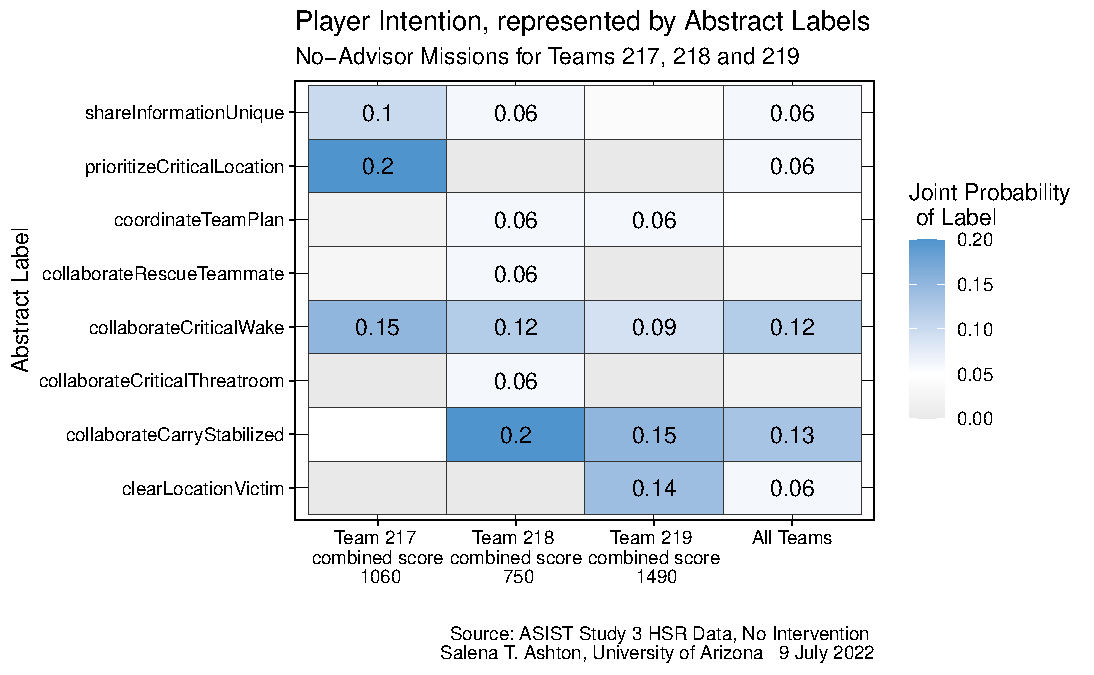
\includegraphics[width=0.9\textwidth]{../images/abstractLabelProbability_STA.pdf}}
    \caption{Player intention (represented by abstract labels) is an unobserved, inferred behavior. Ground-truth question utterances demonstrate team collaboration differently than abstract labels.}
\end{figure}


When we look at the question that was asked, we are able to predict their intentions only part of the time. Though we cannot conclude that questions will always predict intention from this small study, we can see that further research with a larger sample size is warranted. Patterns that emerge include that given question utterance 'requestDestination', the player's intent is more than 80\% likely to be waking a critical victim. Human annotators intuitively agree with this assessment.






Questions Asked, given the Player Intention: Three player intention themes emerge when all possible intentions are filtered for more than 10\%: collaborateCarryStabilized, collaborateCriticalWake, and prioritizeCriticalLocation. When a player's intention is to wake a critical, they are 55\% likely to ask another player to join
 them ('requestDestination'). This observation is trivial because the game rules state that at least two people are needed to wake a critical. However, the previous figure shows the flipped conditions: a player's intention is more than 80\% likely to be waking a critical when 'requestDestination' is asked. When teams collaborate to wake a critical victim, they request or clarify --not suggest or tell-- a teammate to come to a particular destination. ('Clarify' and 'request' infer two-way dialog of commitment creation whereas 'direct' or 'suggest' are creation commitments or demands that do not give the listener a chance to respond.) 








\begin{figure}[h!]
    \centering
    \fbox{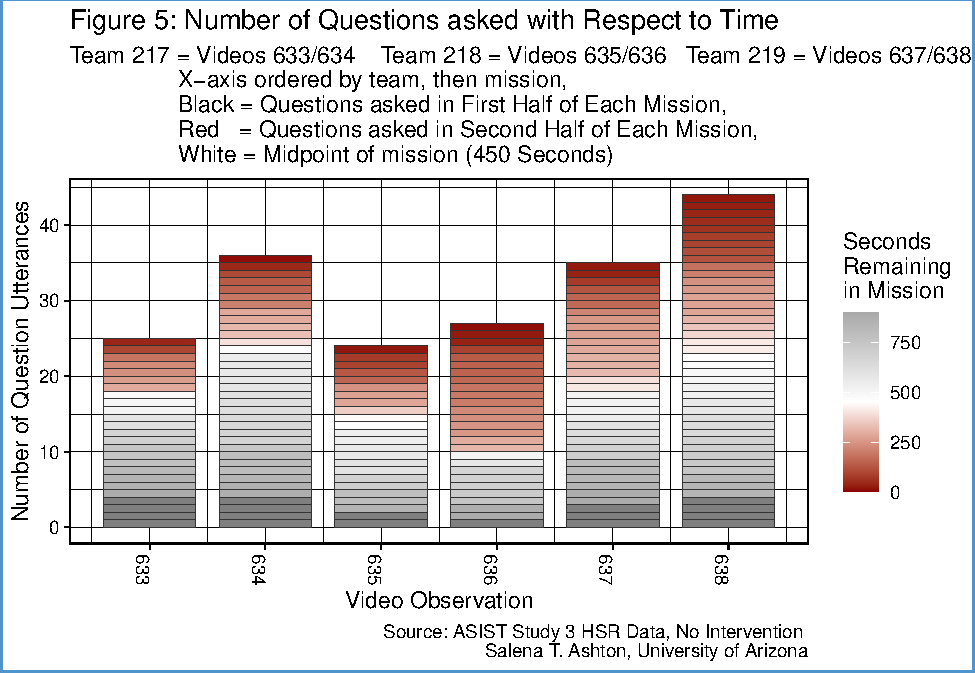
\includegraphics[width=0.9\textwidth]{../images/QuestionTiming_STA.pdf}}
    \caption{Time is displayed as color, where dark gray is at the beginning of the mission and red is toward the end of the mission. Team 218 (videos 635 and 636) asked the
fewest questions, scored the lowest combined points, and asked 66\%
of questions toward the end of the mission. This suggests that teams who score poorly tend to ask fewer questions that focus on collaboration or planning-- and more questions that ask specific task-oriented items toward the end of each mission. Team 3 (videos 637 and 638) asked the most questions and asked questions at a \emph{consistent rate} throughout their missions. This suggests that teams who score higher tend to ask questions at a consistent rate, enabling the exchange of information, building of rapport and team trust, and setting a social convention of asking each other for collaboration or help. }
\end{figure}






\begin{figure}[h!]
    \centering
    \fbox{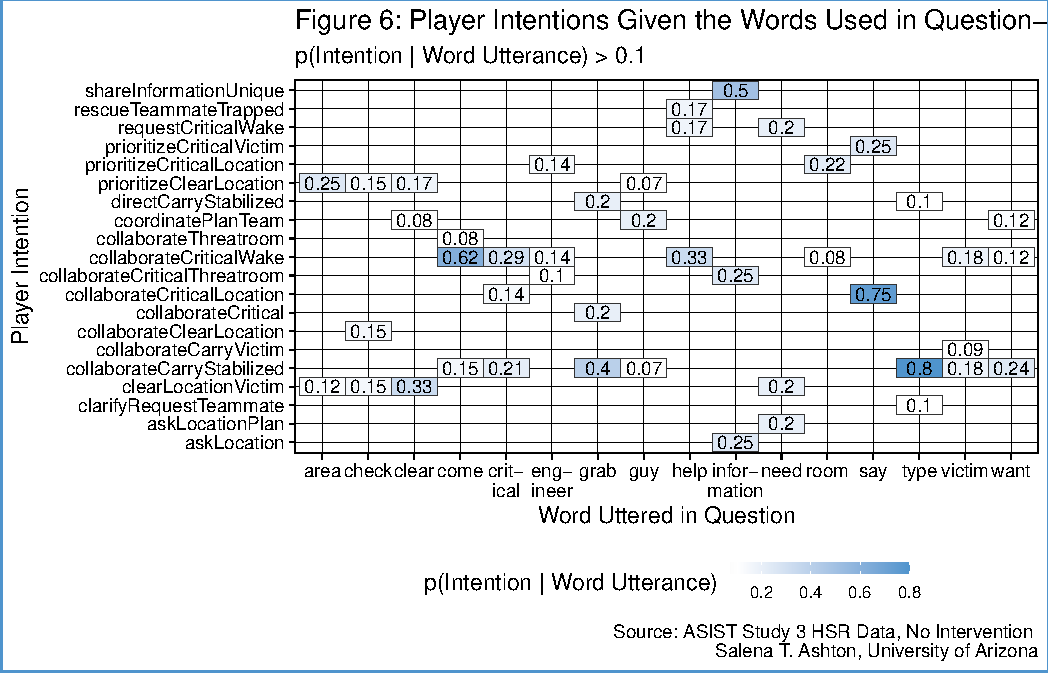
\includegraphics[width=0.9\textwidth]{../images/QuestionUtterances_Link_STA.pdf}}
    \caption{Non-domain-specific words that show collaboration include: say, type, or come. These conclusions were made using the 1 x 1 Bag of Words algorithm and matched to intention by hand. The \textbf{significance} of this figure shows that a priori researcher bias can be harmful when designing a domain. For example, our team previously believed that words like: navigate, location, victim, room, critical and marker were the most important words to look for when inferring player intention. This figures shows that is not the case. A priori research team error: navigate, location, victim, room, critical, marker, or area.}
    \end{figure}
    
   
\begin{comment}
Corrected research team information regarding Player Intention:
\begin{itemize}
    \item 'Come' infers team collaboration for waking up a critical victim
    \item 'Grab' infers team collaboration for carrying victims that have been healed
    \item 'Say' infers team collaboration of locating critical victims
    \item 'Type' infers team collaborating for carrying victims that have been healed
\end{itemize}
\end{comment}




Word Utterance, given Player Intention: Players who work together tend to say  'come', 'say' (stemmed), 'type' or 'want.' When they work together to carry victims, they will most likely say 'type' (or mark) to identify the victim type. As shown, the emergence of a possibly-interesting pattern, especially when non-domain words like 'type' show a strong correlation to specific intentions. The \textbf{significance} of this figure demonstrates how plan-recognition researchers may consider such non domain-specific words when designing a domain.



The ultimate goals of this registration are two-fold: find evidence to (1)
continue the investigation of intent, given a question being asked, using
causal reasoning and other approaches (2) develop algorithms to extract this
intent from utterance transcriptions of player without human annotator
dependency. We believe that emergent categories that result from these 12 video
annotations do *warrant* continued investigation, which would include the
following possible tasks:

\begin{itemize}
    \item Scale for additional data: Ashton is currently building a model that maps words\footnote{Bag of Words and other models, at word and sentence level.} and intentions.
    \item Natural generation model: Use the above model to re-create the labels
        generated by Ashton and Reiffer-Champlin. We will compare these results
        to model labels with the taxonomy developed by ODIN and the Dialog
        Agent at the University of Arizona.
    \item Additional human annotation of data; compare models in earlier stages to these results until the automation of linking intention with natural language is credible and reproducible.
    \item Compare and contrast emerging team ToM from no-intervention observations to high-intervention observations.
    \item Quantitative analyses and causal inference models.
\end{itemize}



\begin{figure}[h!]
    \centering
    \fbox{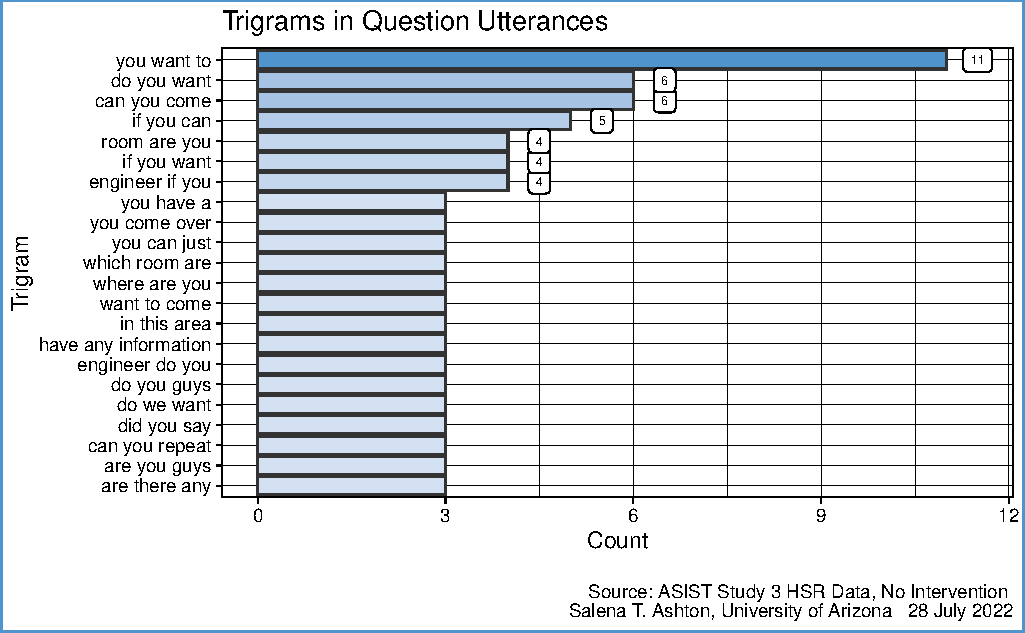
\includegraphics[width=0.9\textwidth]{../images/trigram_Utterances_STA.pdf}}
    \caption{Using the Python package NLTK, I extracted the most common N-grams of the players' question utterances (for all teams, N = 3). When I first did this, there were no interesting patterns. I then removed the "English" library of stopwords to be removed and found the following patterns. This yields exciting potential for further research into the logical argument and flow of player intention. For example, the word "if" shows a conditional statement from one player to another. "If you can..." was a common utterance but it was also a polite imperative, not a request or question. The phrase "do you guys" and "do we want" to not carry as much information about named entities, but it does show ample collaboration of teammates. }
\end{figure}

\begin{figure}[h!]
    \centering    
    \fbox{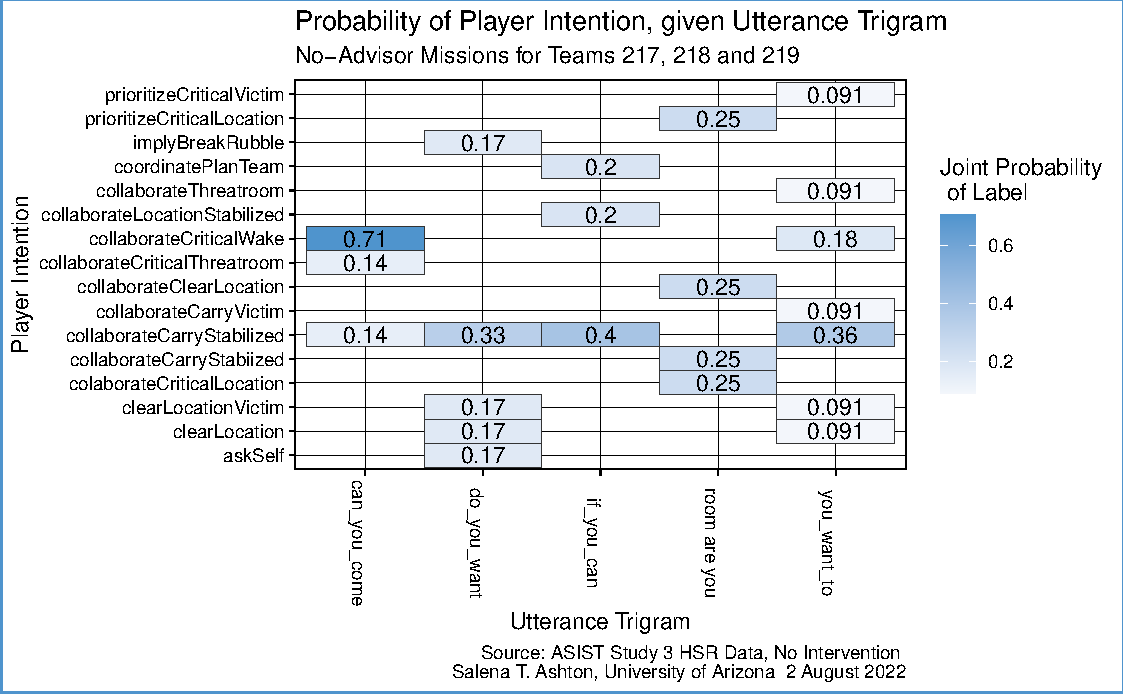
\includegraphics[width=0.9\textwidth]{../images/FINAL_1_trigram_Utterances_STA.pdf}}
    \caption{Probability of Player Intention, given Utterance Trigram}
\end{figure}





\subsection{pasted notes}
a player's intention is more than 80\% likely to be waking a critical when 'requestDestination' is asked. When teams collaborate to wake a critical victim, they request or clarify --not suggest or tell-- a teammate to come to a particular destination. ('Clarify' and 'request' infer two-way dialog of commitment creation whereas 'direct' or 'suggest' are creation commitments or demands that do not give the listener a chance to respond.)


\newpage

In this paper, I have discussed how questions can infer explicitly-stated goals, inferred goals, and how questions are better understood through indirect speech acts. I then use a Search and Rescue scenario within ASIST's Minecraft Environment to evaluate how teammates will ask each other questions in order to make and reach individual and team goals. These goals and player intentions were captured with a robust and vigorous coding process called Grounded Theory, annotated by two completely-autonomous annotators, and reached an unweighted Kappa Cohen score of 0.892. I then investigated these data through a series of visualizations, joint and conditional probabilities, and mapping the data to natural language utterances. This preliminary study has two significant limitations: Only twelve videos were annotated for questions. Future research must include the annotation of many more videos, their questions and non-questions. 

\subsection{Significant findings}
\begin{itemize}
    \item Previous researcher belief that players create intentions around domain-specific words are not supported in this research
    \item Previous top-down domain definition of the Search and Rescue yielded results that were no better than chance. This preliminary study shows several inferences that fair better than chance for player intention, questions asked, and natural language of questions that are asked.
    \item Teams demonstrate collaboration through non domain-specific words like 'come', 'say' and 'type'.
    \item Stops words that are traditionally removed for natural language processing must be considered when infering goals or intentions toward team collaboration. Furthermore, it is these stop words that show the logical inference of such plans.
\end{itemize}

\section{Discussion}

The data collected for this experiment were collected to answer the questions about goal, intention, and question-asking for team players within the virtual environment of a SAR scenario. The data were evaluated to see how teammates will ask each other questions in order to create team goals. These goals and player intentions were captured with a robust and vigorous coding process called Grounded Theory, annotated by two independent and autonomous annotators. Labeling reached an unweighted Kappa Cohen score of 0.892. Using this data, this paper answered three particular questions:
\begin{itemize}
    \item Are teams more likely to score higher when they focus on critical or regular victims?
    \item Do teams who score higher ask more questions?
    \item What types of questions were most frequently asked?
 \end{itemize}

Teams require more collaboration and effort to save critical victims than when saving regular victims; those who ask more questions invite team collaboration and tend to score higher than teams who do not work together. The most common types of questions that teammates asked, given that they scored better than other teams, tended to questions that invited a response. Such questions started with "do", "can", "what", and "which". Common questions which did \textit{not} result in high scores tended to start with "have", "is", and "were". These questions were more about information-seeking than team collaboration.
 
This preliminary study has two limitations: Only twelve videos were annotated for questions. Further research is warranted for the investigation of question-asking, goal-setting, goal-reaching, and team collaboration. Using the current label taxonomy, future research is scaleable and can include the annotation of questions and imperative statements. 



\subsection{Future Research}
I have found that further research is warranted for the investigation of question-asking, goal-setting, goal-reaching, and team collaboration. As a bonus, I have discovered that the stop-words not only hold potential research investigation for the logical flow of such arguments, but can possibly yield new insight into causal inference and reasoning\footnote{It is my intention to continue this line of research for a directed research study in Fall 2022 (Causal Inference) and in Spring 2023 (Comprehensive Qualification Exam for my PhD program in Information Science at the University of Arizona).} It is my hope that the findings of this preliminary study and future research will have significant application toward continued work for the ToMCAT- ASIST program \footnote{Theory of Mind-based Cognitive Architecture for Teams (ToMCAT), Natural Language Generation for Artificial Intelligence and Planning Task \# 7} and for continued study of probabilistic and causal reasoning. 

This future investigation would
address measure ASI-M5: Coordinative Communications to
measure teamwork, include additional video observations for real data in Study
3, and continue our investigation of whether human plans and ToM are best
represented by classical planning or HTN planning.

\newpage






\appendix
\chapter{Domain-specific vocabulary}
\label{ch:vocab}

In this appendix, we list domain-specific vocabulary phrases we provided to the Google Cloud
Speech service as hints for our ASR agent (\autoref{ch:asr}).

\bigskip

{
\footnotesize
\autocols{l}{5}{l}{%
critical,
a critical,
regular,
a regular,
victim,
critical victim,
regular victim,
medic,
medic here,
this is medic,
this is the medic,
engineer,
engineer here,
this is engineer,
this is the engineer,
transporter,
transporter here,
this is transporter,
this is the transporter,
room,
door,
building,
stairs,
window,
floor,
ceiling,
lever,
button,
rubble,
rubble block,
building collapse,
collapse,
move,
open,
close,
push,
toggle,
communicate,
continue,
save,
sight,
question,
agreement,
disagreement,
commit,
clear,
role,
role switch,
search,
change priority,
precedence,
victim,
yellow,
green,
friend,
player,
medkit,
hammer,
stretcher,
map,
red,
blue,
blue suit,
red suit,
green suit,
searching,
strategy,
doorway,
broke,
transported,
transport,
transporting,
agent,
agents,
chat,
die,
double-check,
enter,
found,
hall,
hallway,
help,
locate,
location,
path,
pass,
pick up,
rescue,
A1,
A2,
A3,
A4,
A4A,
B1,
B2,
B3,
B4,
B5,
B6,
B7,
B8,
B9,
C1,
C2,
C3,
C4,
C5,
C6,
C7,
C8,
D1,
D2,
D3,
D4,
E1,
E2,
E3,
E4,
E5,
F1,
F2,
F3,
F4,
F5,
G1,
G2,
G3,
H1,
H2,
H1A,
I1,
I2,
I3,
I4,
I1A,
I2A,
I3A,
I4A,
J1,
J2,
J3,
J4,
K1,
K2,
K3,
K4,
L1,
L2,
L3,
M1,
M2,
M3,
A,
type A,
an A,
an A victim,
B,
type B,
a B victim,
a B,
C,
type C,
a C victim,
a C,
marker,
block,
marker block,
mild,
moderate,
severe,
mild damage,
moderate damage,
severe damage,
meetings,
left side,
right side,
middle,
human resources,
facilities meeting,
project meeting,
security meeting,
zoom2,
zoom2 from office,
zoom,
zoom meeting,
management meeting,
storage reorganization,
lunch,
meeting,
planned meeting,
attendees,
stabilize,
safe block,
safe zone,
diagnose,
injury level,
abrasion,
bone damage,
life threatening,
awaken,
breath bubbles,
destroy,
sledgehammer,
hammer,
first aid kit,
stretcher,
tool,
threat,
threat room,
trapped,
icon,
detection,
device,
detection device,
victim detection device,
north zone,
south zone,
zone,
relocate,
building structure,
news room,
updates,
news room updates,
grid,
SOS,
help me,
help me here,
ground,
navigate,
approach
}}


% hypotheses?
% - TMM model can predict behavior
% - TMM agent interventions improve performance
% - Closed loop communication is predictive of team performance
\printbibliography
\end{document}
